%===============================================================================
% ifacconf.tex 2025-07-31 jpuente  
% 2022-11-11 jpuente change length of abstract
% 2025-07-31 jldiez added section on the use of AI
% Template for IFAC meeting papers
% Copyright (c) 2025 International Federation of Automatic Control
%===============================================================================
\documentclass{ifacconf}

\usepackage{graphicx}      % include this line if your document contains figures
\usepackage{natbib}        % required for bibliography
\usepackage{xcolor}
\usepackage{subcaption}
\usepackage{siunitx}
\usepackage{amsmath,amssymb,amsfonts} 

\newcommand{\TODO}[1]{
\textcolor{red}{\textbf{TODO} #1}
}
%===============================================================================
\begin{document}
\begin{frontmatter}

\title{\textcolor{red}{Style for IFAC Conferences \& Symposia: Use Title Case for
  Paper Title}} 
% Title, preferably not more than 10 words.

\author[First,Second]{Alessandra Elisa Sindi Morando} 
\author[Second]{Jossué Cari\~no}
\author[Second]{Pedro Castillo} 
\author[First]{Roberto Sacile}
\author[First]{Enrico Zero}

\address[First]{
   \textit{University of Genoa}, Genoa, Italy \\
   alessandra.elisa.sindi.morando@edu.unige.it, roberto.sacile@unige.it, enrico.zero@dibris.unige.it
}
\address[Second]{
   \textit{Université de technologie de Compiègne}, CNRS, Heudiasyc, Compiègne, France \\
   alessandra-elisa-sindi.morando@utc.fr, \{jossue.escobar, pedro.castillo\}@hds.utc.fr
}

\begin{abstract}                % Abstract of 50--100 words
\textcolor{red}{\dots}
\end{abstract}

\begin{keyword}
   \textcolor{red}{\dots}
   %Five to ten keywords, preferably chosen from the IFAC keyword list.
\end{keyword}

\end{frontmatter}
%===============================================================================

\section{Introduction}
Multi-agent systems (MASs) are nowadays used in a variety of applications from as
they can perform complex tasks, which would otherwise impossible for a single robot.
This is even more the case when considering heterogeneous fleet where the strenghts
of one type of robot can compensate for the limitations of another.
For example, to monitor a large area, multiple ground agents can move from one point 
to another being supervised from above by a drone with a wide field of view.
To deepen the subject and understand both the potential tasks and challenges of MASs,
the reader can refer to the work of~\cite{Maldonado2024}.

One of the fundamental cooperative tasks when working with multi-agents is formation
control.
This topic has been studied for years.
For example, already~\cite{LEE200985} already proposed
a decentralized control algorithm for a team of two-wheeled robots 
to achieve achieve a geometric pattern.
However, formation control remains an hot challenging topic to this day.
\cite{TRAN2021100117} experimentally validated a robust distributed control 
based on negative imaginary systems consensus theory, using both ground robots and
an air-ground fleet.
In the work of~\cite{GULER2023105492}, each agent computes its control action 
in a leader-follower manner using local extended Kalman filter's estimates to 
achieve a desired shape together with other wheeled robots and a drone.
An optimal distributed formation control algorithm for double-integrator multi-agents
has been presented and validated through simulations by~\cite{Huang2023}.
\cite{Aditya2023} defined the formation problem for a group of double-integrator agents 
as a discrete-time game whose solution is given by a state-dependent Riccati equation.
A robust distributed consensus controller is presented by~\cite{Restrepo2023}
to address the rendezvous problem and applied in simulation to a swarm of drones.
In the recent years, reinforcement learning has used in many areas including 
formation control. 
\cite{WANG20208150} addressed multi-particle formation control by combining 
graph attention networks and multiple long short-term memories to achieve the 
desired shape and avoid collisions respectively.
A position and an orientation robust controllers based on reinforcement learning 
are proposed and validated through simulations by~\cite{Zhong2025} for the formation 
of a term of quadrotors.

In this context is placed this work which proposes a novel formation control scheme
for a team consisting of a quadcopter and two unicycles, as show in Fig.~\ref{fig:summary_image}.
\begin{figure}
    \centering
    % trim = left bottom right top (in points or any unit)
    % clip = true ensures the parts outside the box are hidden
    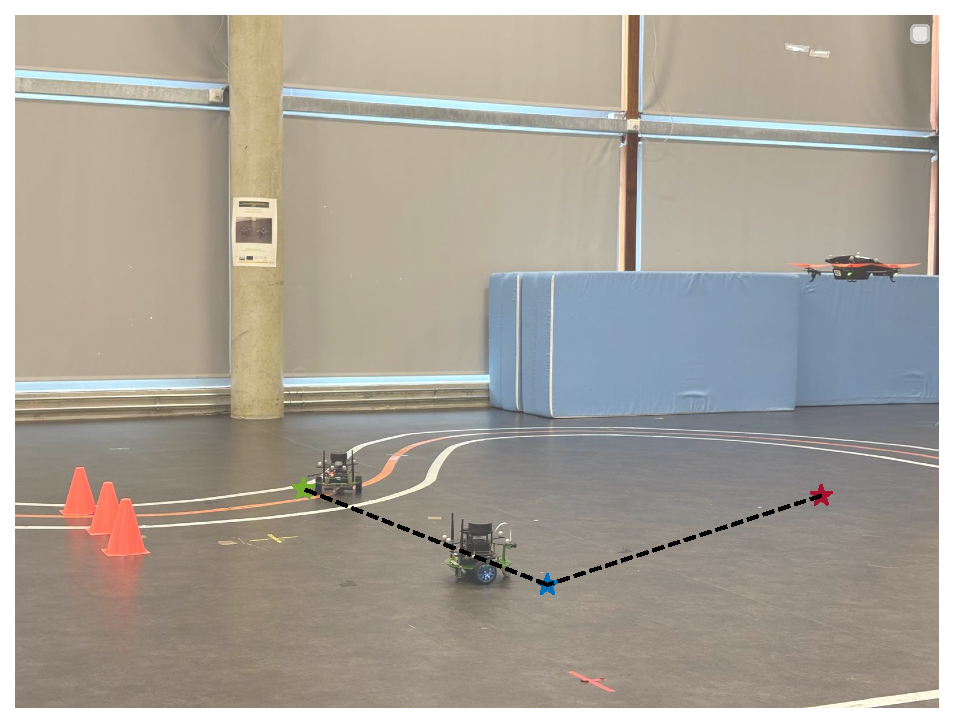
\includegraphics[width=0.9\columnwidth, trim=10 50 15 110, clip]{images/output.pdf}
    \caption{This paper proposes a formation control for a heterogeneous fleet to attain a desired shape despite obstacles.}
    \label{fig:summary_image}
    \vspace{-0.1cm}
\end{figure}
When addressing the multi-agent formation, there are two main challenges to solve: 
achieving the desired shape and avoiding collisions.
On one hand, for the first challenge, a distributed controller combining Feedback 
Linearization (FL) and an optimal linear controller based on Linear Matrix 
Inequalities (LMIs) is presented.
LMIs are a powerful mathematical tool used in many applications among which also 
formation control.
In the work of~\cite{Trejo2023}, an LMI is solved to design the controller 
and observer gains, guaranteeing stable formation flight for a group of quadcopters.
~\cite{Deshpande2011} propose a formation control with artificial 
fixed delays for multiple double-integrators and 
verify the asymptotic stability of the scheme by checking 
the solvability of an LMI.
~\cite{Semsar2009} present an LMI formulation of the LQR problem 
to guarantee stable state consensus with an optimal control effort 
in a multi-agent system.
On the other end, to avoid collision avoidance, the chosen solution is 
Artificial Potential Field (APF).
In analogy with a particle moving in an electrostatic or gravitational
field, virtual repulsive force fields are simulated to ward off the robot
from an obstacle.
This approach has been widely used in formation control of ground vehicles,
see for example the work of~\cite{Yongshen2018}.
However, in more recent works, e.g.~\cite{HAN2024106105} and~\cite{Piet2025Control},
APFs are employed to navigate around obstacles and prevent collisions 
while attaining the desired shape.
% \textcolor{red}{
% \begin{itemize}
%    %  \item survey on multi-agent systems~\cite{Maldonado2024}
%    %  \item other works on air-ground cooperation:
%    %  \item works on obstacle avoidance and formation:
%    %  ~\cite{WANG20208150},
%    %  ~\cite{TRAN2021100117} (air-ground),
%    %  ~\cite{GULER2023105492}(air-ground, adaptive distributed leader-follower controller for formation),
%    %  ~\cite{Huang2023}(optimal algoritm, as me, and control barrier function),
%    %  ~\cite{Restrepo2023}(UAVs formation, collision vaoidance guaranteed with constraints),
%    %  ~\cite{Aditya2023}(double integrator Riccati equation for formation and collision avoidance)
%    %  ~\cite{LEE200985},
%    % \item LMI:
%    % ~\cite{Deshpande2011}(LMI  double integrator formation),
%    % ~\cite{Trejo2023}(use LMI to find controller gains for UAVs formation), 
%    % ~\cite{Semsar2009}(LMI to optimal consensus multi-agent)
%    %  \item other works with APF:
%    %  ~\cite{Yongshen2018}(applied to UGVs),
%    %  ~\cite{Piet2025Control, HAN2024106105} (both applied to drones)
%     \item previous work:~\cite{Morando2025SOSE}
% \end{itemize}
% }

This paper represents the continuation of the previous work by~\cite{Morando2025SOSE},
where a control architecture combining Feedback Linerarization (FL), 
a robust LMI-based controller and APFs was proposed 
and validated through simulations for 
the formation of three unicycles.
The successive developments sought to manage the challenge
of a heterogeneous team (replacing a ground vehicle with a quadcopter)
by adapting the methodology and then experimentally validating 
the new solution.
The contributions of this work are: a) a controller involving FL, a LMI-based controller and APFs 
is presented for the stable formation of an air-ground fleet;
b) the proposed controller has been validated through MATLAB Simulink
simulations and a comprensive set of experiments in an indoor arena, including both static
and dynamic obstacle scenarios.
The remainder paper is structured as follows. 
In Section~\ref{sec:heterogeneous_fleet_modeling}, 
the mathematical model used to describe the team is stated.
The proposed formation controller is detailed in Section~\ref{sec:formation_controller}.
The simulations and the experiments results are reported and analyzed
in Section~\ref{sec:simulation_results} and 
in Section~\ref{sec:experimental_validation} respectively.
Finally, conclusions are drawn in Section~\ref{sec:conclusion}.

\section{Heterogeneous Fleet Modeling}
\label{sec:heterogeneous_fleet_modeling}
In this section, the dynamics of the agents composing the team
(i.e., of the two unicycles and the quadrotor, as shown in Fig.~\ref{fig:airground-fleet}.)
are described and adapted to then apply the LMI approach.
\begin{figure}
    \centering
   %  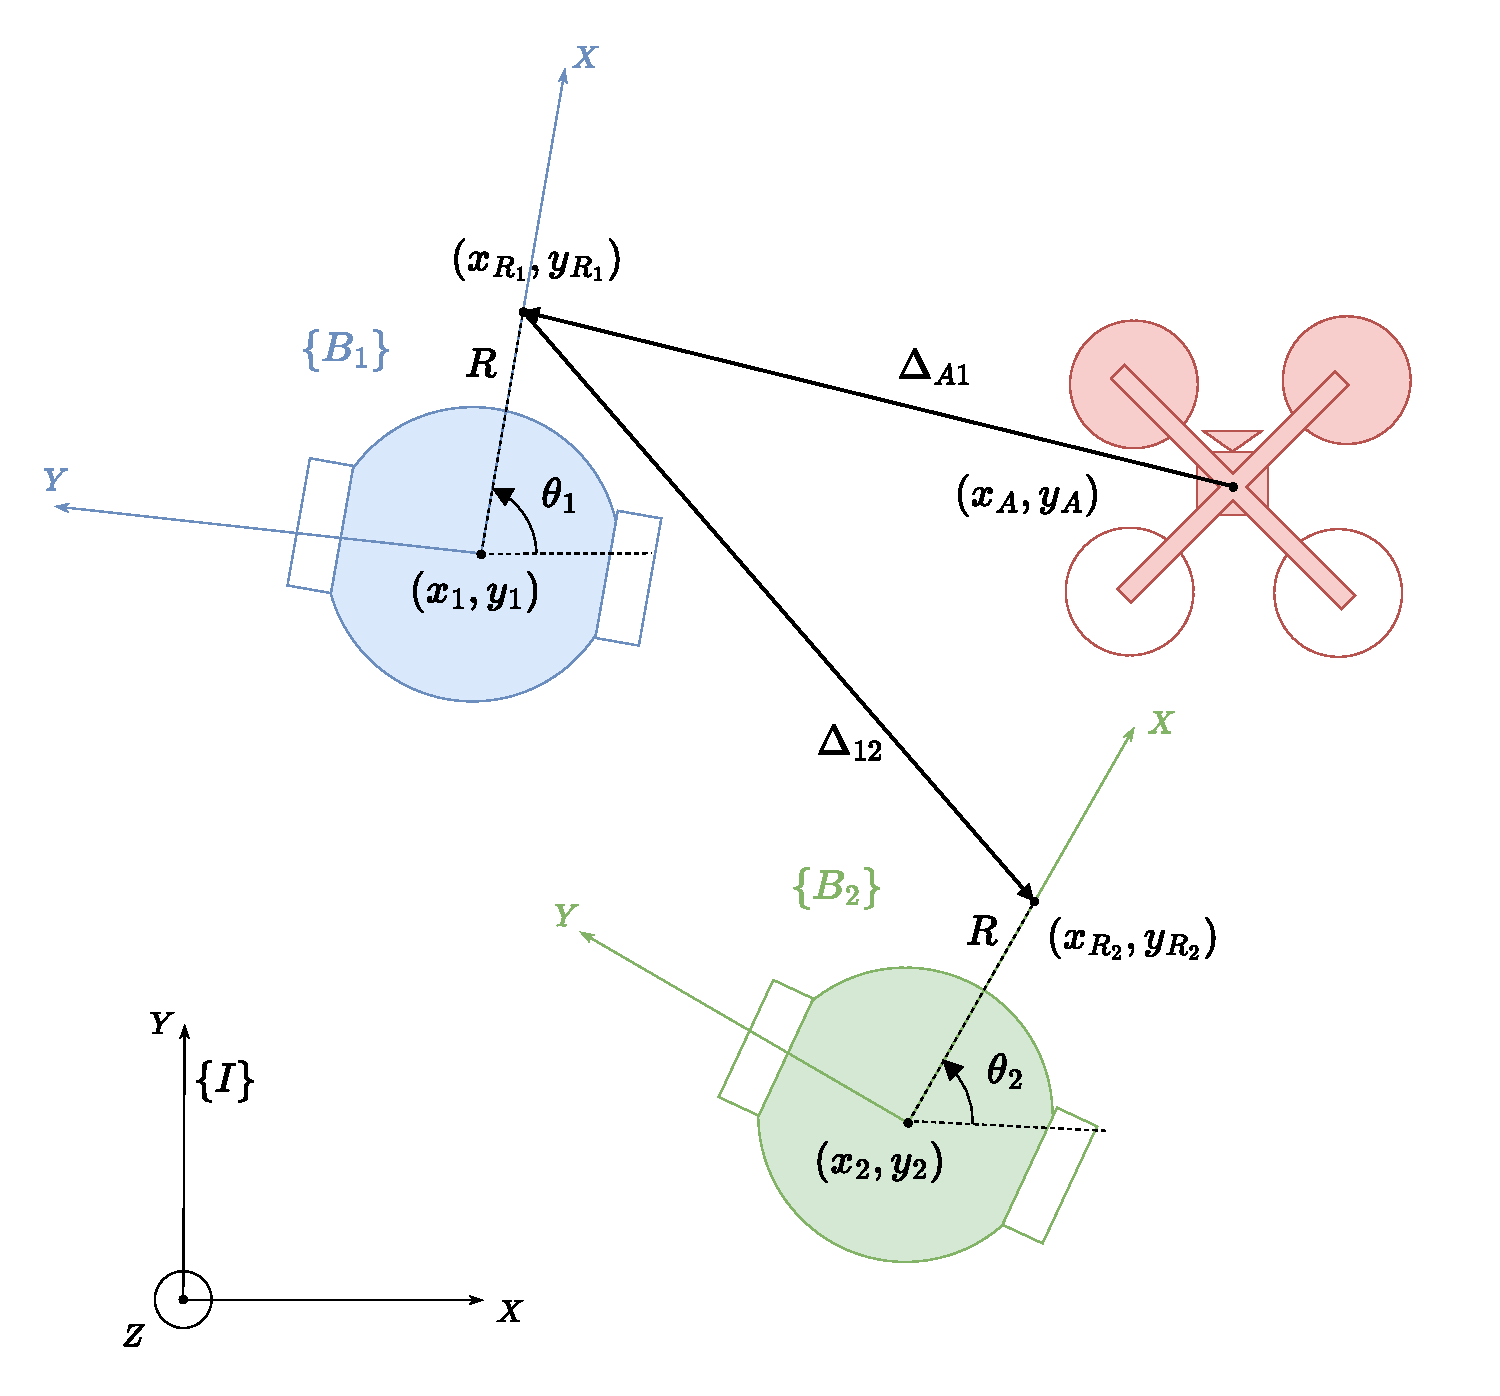
\includegraphics[height=6cm]{images/heterogenous_fleet.pdf}
    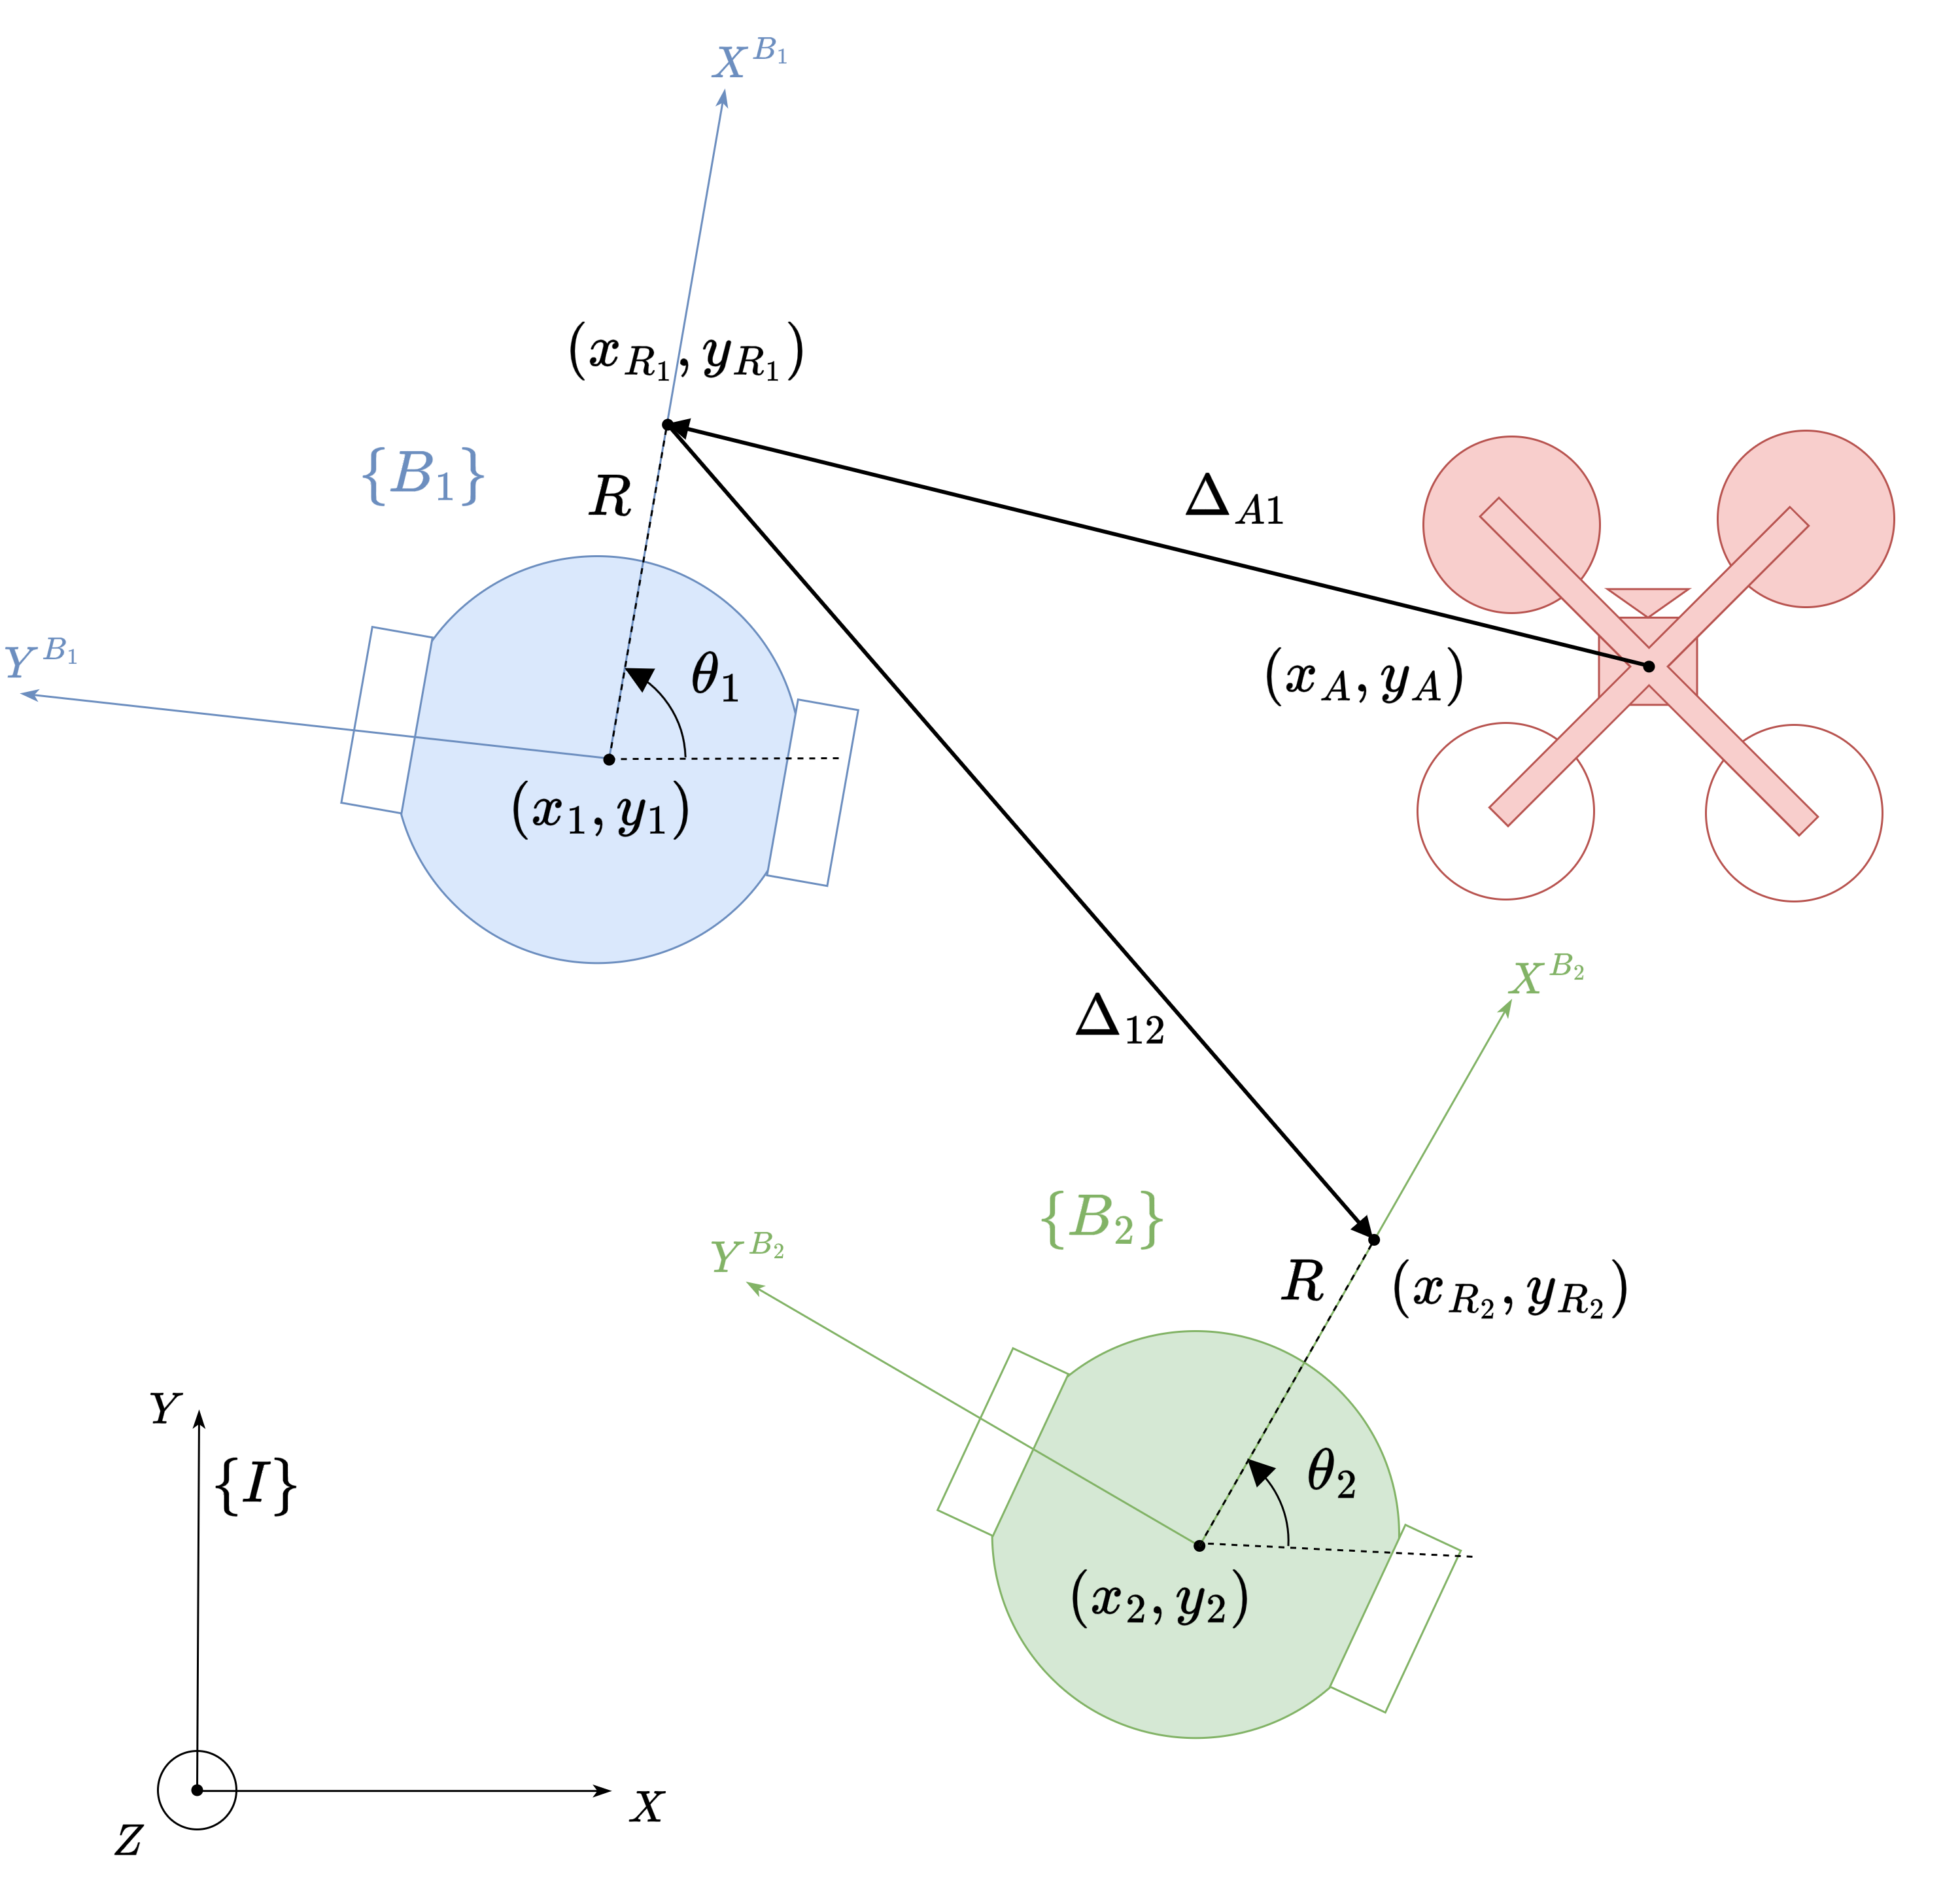
\includegraphics[height=6.1cm]{images/heterogenous_fleet_PNG300_2.png}
    \caption{Air-ground heterogeneous fleet.}
    \label{fig:airground-fleet}
\end{figure}
The well-known kinematic model of a two-wheeled ground robot $G_i$ is
\begin{equation}
    \begin{cases}
        \dot{x}_i &= v_i \, \cos\theta_i \\
        \dot{y}_i &= v_i \, \sin\theta_i \\
        \dot{\theta}_i &= \omega_i
    \end{cases}
    \label{eq:unicycle_i_t-model}
\end{equation}
where $(x_i, y_i, \theta_i)$ is the pose of the agent 
and $(v_i, \omega_i)$ are the linear and
angular velocities respectively.
The equations~\eqref{eq:unicycle_i_t-model} describing the motion of the center of rotation are non-linear.
But still, if a point located at distance $R > 0$ from 
$(x_i, y_i)$ denote as $({x}_{R_i}, {y}_{R_i})$, is 
considered and new virtual inputs are defined $(u_{i,x},u_{i,y})$, 
the dynamics become linear:
\begin{equation}
    \begin{cases}
        \dot{x}_{R_i} = u_{i,x} \\
        \dot{y}_{R_i} = u_{i,y} \\
    \end{cases}
\end{equation}
Moving on to the drone, as in the formation problem deals with the $(X,Y)$-dynamics, some simplifying hypothesis have been made.
First, let us assume that there is an inner attitude controller.
Hence, the focus is only on the translational dynamics which are:
\begin{equation}
    \begin{cases}
        m\ddot{x}^F_A = - T \sin \theta \\
        m\ddot{y}^F_A = T \cos \theta \sin \phi \\
        m\ddot{z}^F_A = T \cos \theta \cos \phi  - m\, g\\
    \end{cases}
\end{equation}
Let analyze the equations with the help of Fig.~\ref{fig:drone_roll_pitch_frames}.
The state $({x}^F_A,{y}^F_A,{z}^F_A)$ represents the position of the drone w.r.t. the inertial frame $\{F\}$.
The frame $\{F\}$ has been used instead of $\{I\}$ to be aligned with the framework employed 
to implement the controller for the drone, see Section~\ref{sec:experimental_validation}.
The angles $\phi$ and $\theta$ are the roll and pitch Euler angles 
of the body frame $\{B\}$ (fixed to the drone) relative to the inertial
frame $\{F\}$.
Ignoring the small body forces, the only forces acting on the drone are 
the trust produced by the motors $T$ along the $k^B$ direction and 
the gravity $mg$ along the $-k^F$ direction.
\begin{figure}
    \centering
    \begin{subfigure}{0.31\columnwidth}
        % trim = left bottom right top (in points or any unit)
        \hspace{0.5cm}
        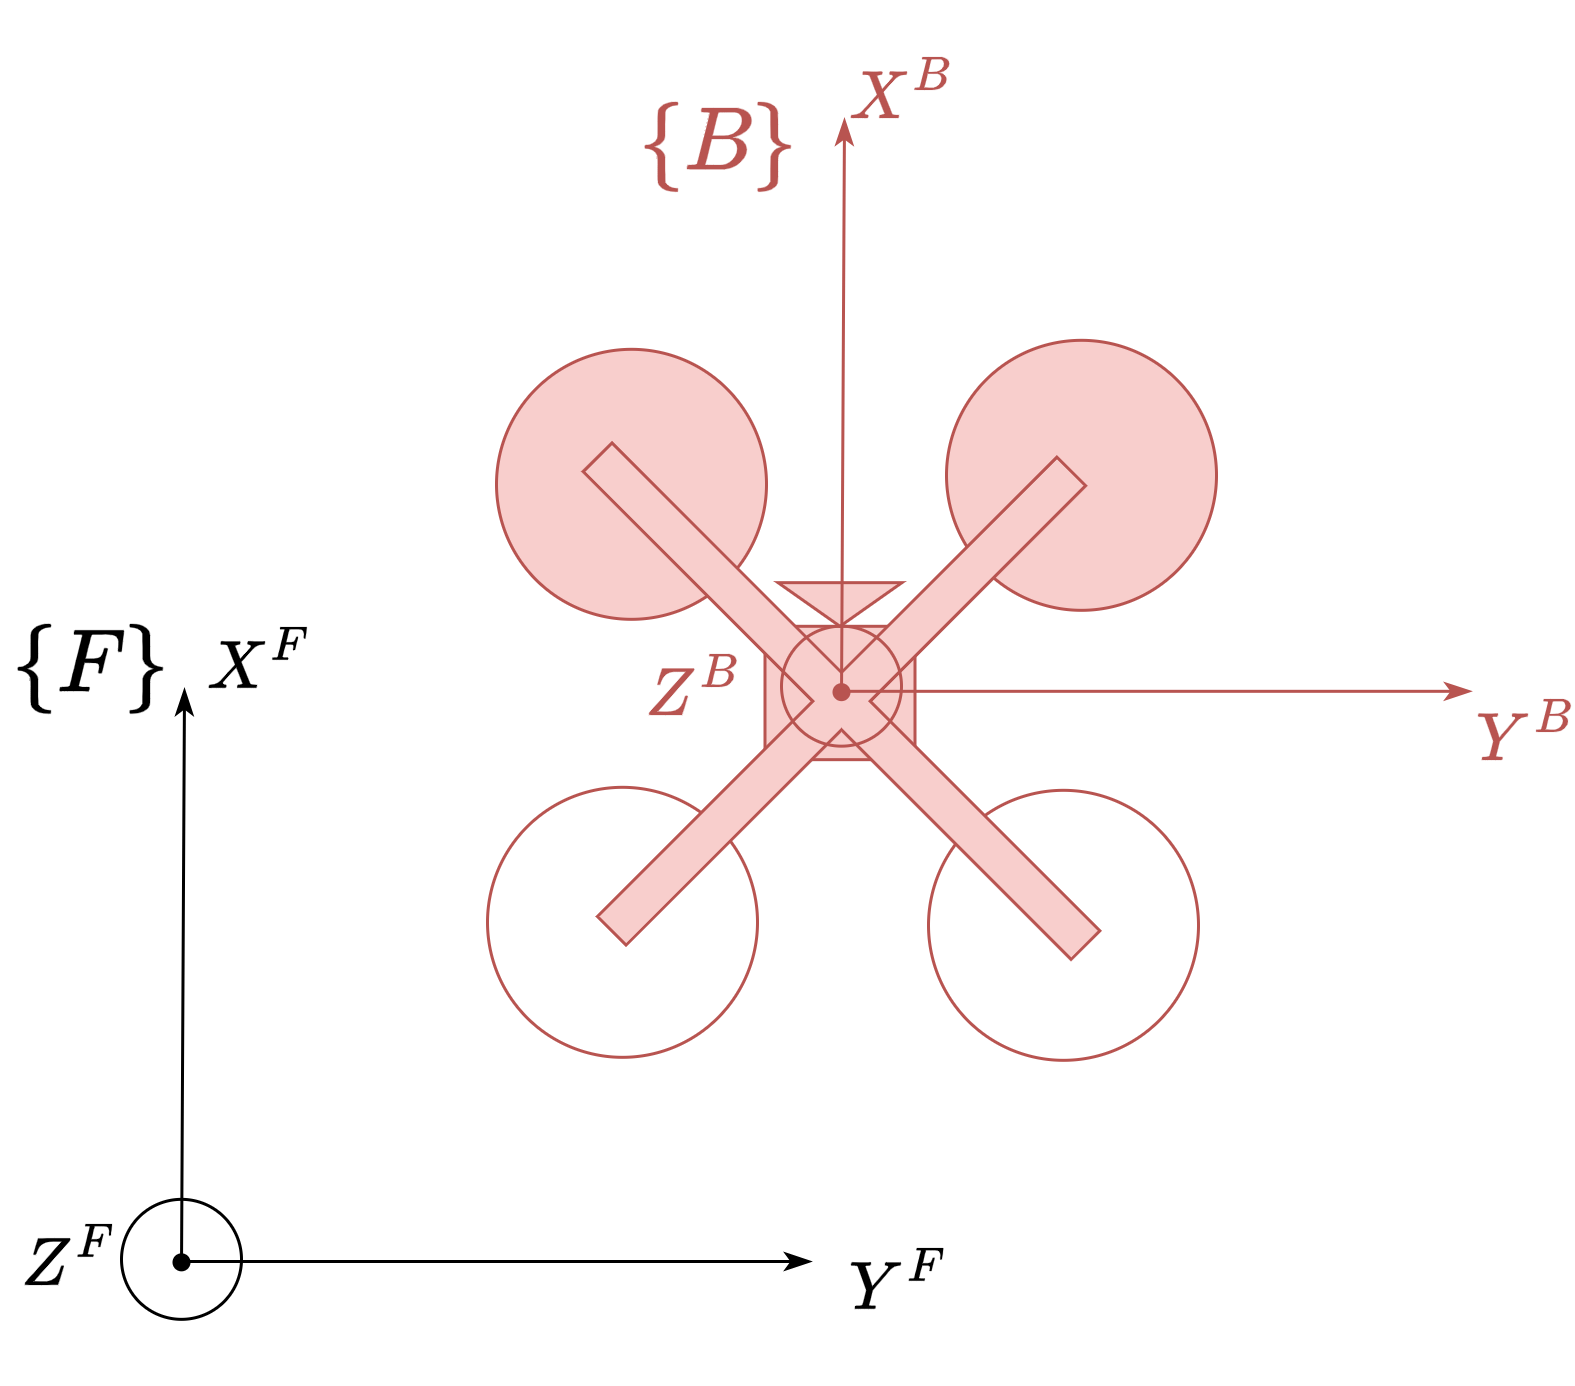
\includegraphics[trim={0.8cm 2cm 0cm 2cm}, clip, width=3cm]{images/drone_fromAbove2.png}
        % \caption{Drone's body frame $B$ and FL-AIR frame $F$.}
    \end{subfigure}
    \hfill
    \begin{subfigure}{0.31\columnwidth}
        \hspace{0.5cm}
        % 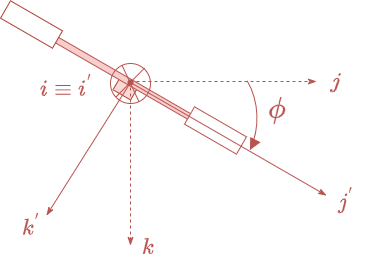
\includegraphics[trim={0.8cm 0.4cm 0cm 0.5cm}, clip, width=3cm]{images/drone_roll.png}
        % \vspace{-1.3cm}
        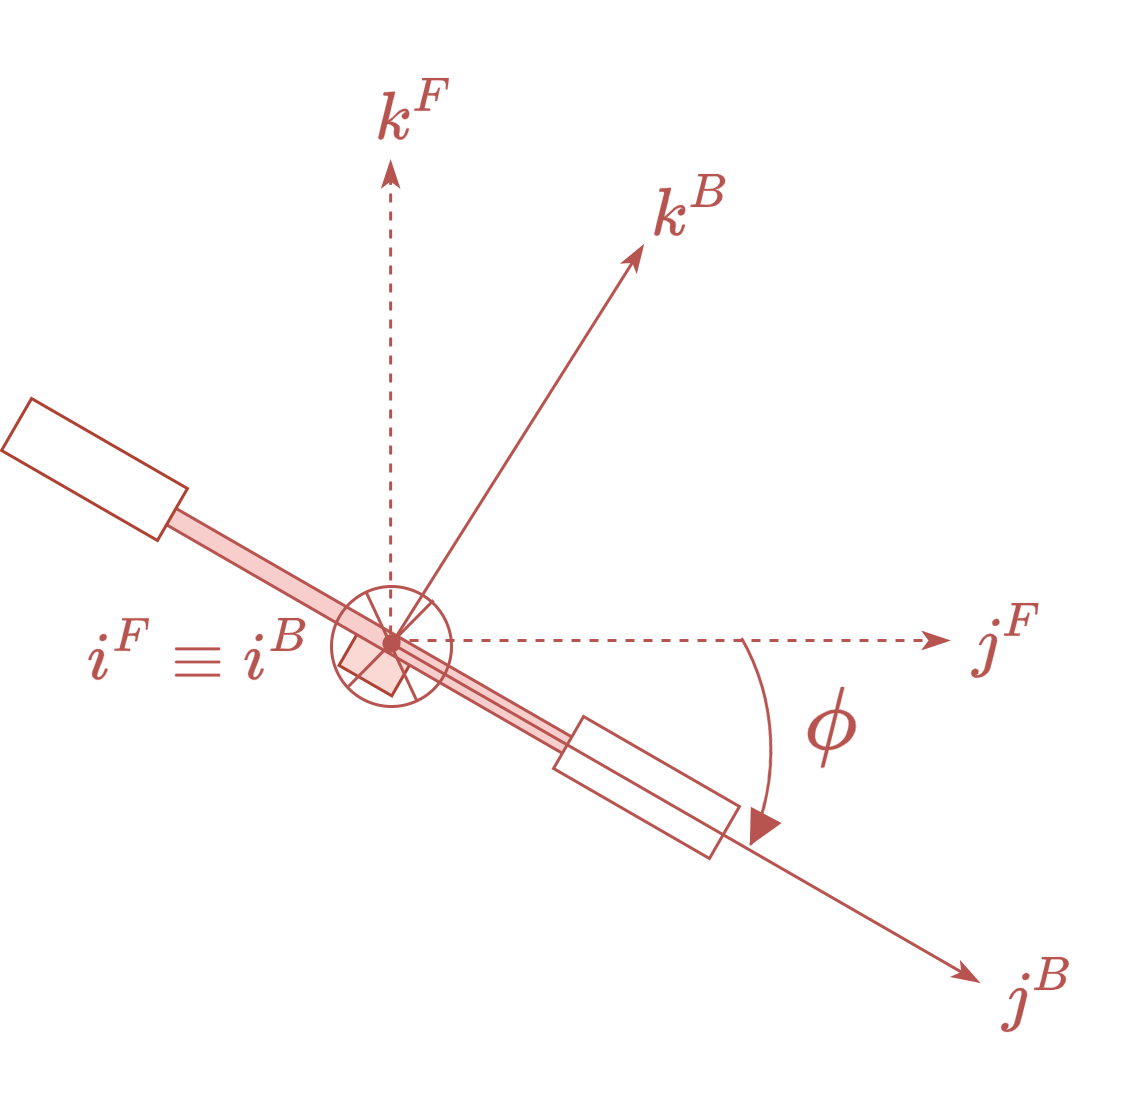
\includegraphics[trim={0cm 0cm 0.5cm 0cm}, clip, width=3cm]{images/drone_roll3.png}
        % \vspace{0.7cm}
        % \caption{Roll $\phi$ w.r.t  the frame $B$.\\}
    \end{subfigure}
    \hfill
    \begin{subfigure}{0.31\columnwidth}
        \hspace{0.3cm}
        \vspace{0.5cm}
        % 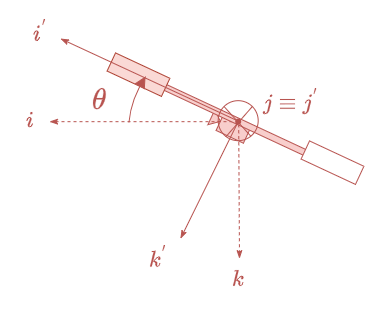
\includegraphics[trim={0cm 0cm 0.5cm 0cm}, clip, width=3cm]{images/drone_pitch.png}
        % \vspace{0.9cm}
        % \vspace{-0.01cm}
        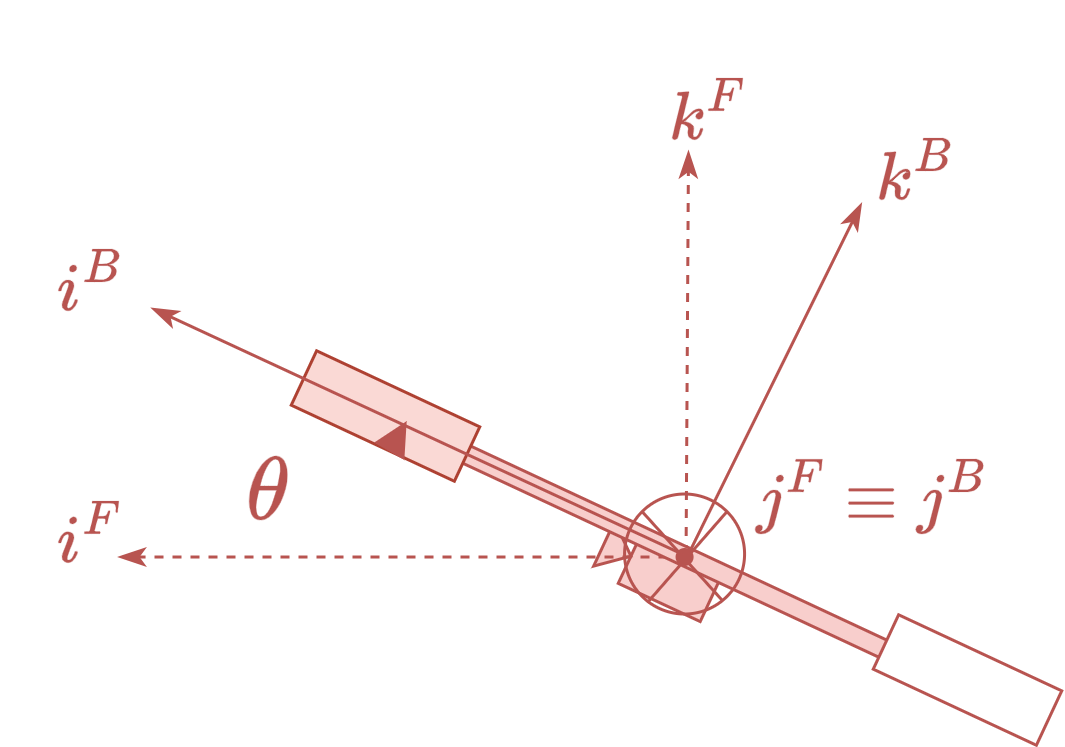
\includegraphics[trim={0.8cm 0.1cm 0cm 0.5cm}, clip, width=3cm]{images/drone_pitch2.png}
        % \vspace{0.1cm}
        % \vspace{0.9cm}
        % \caption{Pitch $\theta$ w.r.t  the frame $B$.\\}
    \end{subfigure}
    \caption{Quadcopter's roll $\phi$ and pitch $\theta$ angles.} 
    \label{fig:drone_roll_pitch_frames}
\end{figure}
Let suppose that the $Z$-controller 
\begin{equation}
    T = (r_1 + mg) / (\cos \phi \cos \theta)
\end{equation}
is such that the drone's mass is compensated in a short time
by $r_1$, i.e. $r_1 \to 0$.
This implies that the $(x,y)$-dynamics will not include the mass of the drone,
as the $Z$-controller already compensated it.
Finally, let us make the hypothesis that the roll and pitch angles 
are small, i.e. $\phi,\theta \approx 0$.
Then, the translational dynamics simplify to 
\begin{equation}
    \begin{cases}
        \ddot{x}^F_A = -g\theta \\
        \ddot{y}^F_A = g\phi
    \end{cases}
    \label{eq:drone_t-model}
\end{equation}
At this point, all the agents can be described by the linear models
\eqref{eq:unicycle_i_t-model} and~\eqref{eq:drone_t-model}.
To define the formation problem, let us introduce the quantities
\begin{subequations}
    \begin{equation}
        \Delta_{A1} = \begin{bmatrix}
            \Delta_{A1,x} & \Delta_{A1, y}
        \end{bmatrix}^T 
    \end{equation}
    \begin{equation}
        \Delta_{A1,x} = x_{R_1} - x_A = x_{R_1} - y^F_A \  
    \end{equation}
    \begin{equation}
        \Delta_{A1,y} = y_{R_1} - y_A = y_{R_1} - x^F_A
    \end{equation}
\end{subequations}
with $(x_A, y_A)$ the position of the drone w.r.t the inertial frame $\{I\}$,
\begin{subequations}
    \begin{equation}
        \Delta_{12} = \begin{bmatrix}
        \Delta_{12,x} & \Delta_{12, y}
    \end{bmatrix}^T 
    \end{equation}
    \begin{equation}
        \Delta_{12,x} = x_{R_2} -  x_{R_1}, \ 
        \Delta_{12,y} = y_{R_2} -  y_{R_1}
    \end{equation}
\end{subequations}
the desired inter-distances $ \Delta^d_{A1}$ and $\Delta^d_{12}$,
 and the desired position of the drone $(x^d_A, y^d_A)$ w.r.t the inertial 
 frame $\{I\}$ (constant over time).
The overall dynamics of the formation's errors are as follows
\begin{equation}
\begin{cases}
    \ddot{e}_{A,x} = - g \theta \\
    \ddot{e}_{A,y} = g \phi \\
    \dot{e}_{\Delta_{A1,x}} = u_{1,x}  - \dot{e}_{A,y} \\
    \dot{e}_{\Delta_{A1,y}} = u_{1,y}  - \dot{e}_{A,x} \\
    \dot{e}_{\Delta_{12, x}} = u_{2,x}  - u_{1,x} \\
    \dot{e}_{\Delta_{12, y}} = u_{2,y}  - u_{1,y}
\end{cases}
\label{eq:airground-continous_time-sys}
\end{equation}
with 
\begin{equation}
e_{A,x} = x^F_A - y^d_A, \ e_{A,y} = y^F_A - x^d_A
\end{equation}
\begin{equation}
e_{\Delta_{A1,x}} = \Delta_{A1,x} - \Delta^d_{A1,x}, \ 
e_{\Delta_{A1,y}} = \Delta_{A1,y} - \Delta^d_{A1,y}
\end{equation}
\begin{equation}
e_{\Delta_{12,x}} = \Delta_{12,x} - \Delta^d_{12,x}, \ 
e_{\Delta_{12,y}} = \Delta_{12,y} - \Delta^d_{12,y}
\end{equation}
Let us define the state and control vectors as follows
\begin{subequations}
    \begin{equation}
        \footnotesize
        \boldsymbol{e}^T = \begin{bmatrix}
            e_{A,x} & \dot{e}_{A,x} & e_{A,y} & \dot{e}_{A,y} 
            & e_{\Delta_{A1,x}} & e_{\Delta_{A1,y}}
            & e_{\Delta_{12,x}} & e_{\Delta_{12,y}}
        \end{bmatrix}
    \end{equation}
    \begin{equation}
        \boldsymbol{u}_A = \begin{bmatrix}
            \phi  \\ \theta 
        \end{bmatrix}, \
        \boldsymbol{u}_1 = \begin{bmatrix}
            u_{1,x} \\ u_{1,y}
        \end{bmatrix}, \ 
        \boldsymbol{u}_2 = \begin{bmatrix}
            u_{2,x} \\ u_{2,y}
        \end{bmatrix}, 
        \boldsymbol{u} = \begin{bmatrix}
            \boldsymbol{u}_A \\ \boldsymbol{u}_1 \\  \boldsymbol{u}_2
        \end{bmatrix}
        \label{eq:airground-continous_time-controls}
    \end{equation}
\end{subequations}
Hence, the heterogeneous fleet's dynamics can be written in a matrix form:
\begin{equation}
    \dot{\boldsymbol{e}} = A \boldsymbol{e} + B \boldsymbol{u}
\end{equation}
By discretizing with sampling time $\Delta T$ using the Euler method:
\begin{equation}
    \boldsymbol{e}(k+1) = A_d \boldsymbol{e}(k) + B_d \boldsymbol{u}(k) 
    \label{eq:airground-fleet-z}
\end{equation}
with $A_d = I + \Delta T A $ and $B_d = \Delta T B$.
To model real-world disturbances, it is assumed 
that an addictive zero-mean disturbance $\boldsymbol{d}(k)$
is acting on the input channel, i.e.
\begin{equation}
    \boldsymbol{e}(k+1) = A_d \boldsymbol{e}(k) + B_d \boldsymbol{u}(k) + B_d \boldsymbol{d}(k)
    \label{eq:airground-fleet-z}
\end{equation}
Let us make the following hypothesis: 
a) the drone knows its position;
b) the robot $G_1$ knows its position w.r.t the quadcopter;
c) the robot $G_2$ knows its position w.r.t the other agent $G_1$;
d) all unicycles are aware of their distance from any obstacles on the ground;
e) a hierarchy is defined between the ground robots: $G_1$ has the priority over $G_2$.
\section{Formation Controller}
\label{sec:formation_controller}

This section aims to detail the proposed formation controller.
The two crucial issues, formation maintenance and collision avoidance, 
are addressed respectively in the next two subsections.


\subsection{Formation Maintenance: an LMI Approach}
The first goal is to ensure the robots achieve the desired shape 
while using only local measurements 
and counteracting the worst-case disturbance.
Based on the previous hypotheses, the measurements of 
each agent are as follows:
\begin{subequations}
    \begin{equation}
    \boldsymbol{z}_A = \begin{bmatrix}
        e_{A,x}  \\ e_{A,y} \\ \dot{e}_{A,x} \\ \dot{e}_{A,x}
    \end{bmatrix}= C_A \, \boldsymbol{e}
\end{equation}
\begin{equation}
    \boldsymbol{z}_1 = \begin{bmatrix}
        e_{\Delta_{A1,x}} \\ e_{\Delta_{A1,y}}
    \end{bmatrix} = C_1 \, \boldsymbol{e}, \  
     \boldsymbol{z}_2 = \begin{bmatrix}
        e_{\Delta_{12,x}} \\ e_{\Delta_{12,y}}
    \end{bmatrix} = C_2 \, \boldsymbol{e}
\end{equation}
\label{eq:airground-continous_time-measurement}
\end{subequations}
with $C_A$, $C_1$, and $C_2$ the measurement matrices of the three.
The idea is to formulate the robust formation control 
problem as a dynamic game between two players: 
one is the control action and the other opponent is 
the ``nature''.
In the proposed solution, at each time step $k$ the control 
action to be applied at the next step $\boldsymbol{u}(k)$
is obtained by solving the following min-max problem 
defined over a one-step horizon.
\begin{equation}
\footnotesize
\begin{aligned}
    \min_{\boldsymbol{u}(k)} \max_{\boldsymbol{e}(k) \neq 0} &  \quad 
    \frac{J(k)}{\left\lVert \boldsymbol{e}(k)\right\rVert^2_2} \\
    \textrm{s.t.} \  &\boldsymbol{z}_i(k) = C_i \, \boldsymbol{e}(k) \\
    \quad & \boldsymbol{u}_{i}(k) = \boldsymbol{\mu}_i(\boldsymbol{z}_i(k)) \quad i \in \{A,1,2\} \\
\end{aligned}
\end{equation}
with
\begin{equation}
    \footnotesize
    J(k) = \boldsymbol{u}(k)^TQ_u\boldsymbol{u}(k)+\boldsymbol{e}(k+1)^TQ_e\boldsymbol{e}(k+1)+\boldsymbol{e}(k)^TQ_e\boldsymbol{e}(k)   
\end{equation}
The cost function can be rewritten by substituting the evolution model 
equation~\eqref{eq:airground-fleet-z}.
\begin{equation}
\footnotesize
    J(k) = \begin{bmatrix}
        \boldsymbol{e}(k) \\ \boldsymbol{u}(k)
    \end{bmatrix}^T \begin{bmatrix}
        Q_e + A_d^T Q_e A_d & A_d^T Q_e B_d \\ 
        B_d^T Q_e A_d & Q_u + B_d^T Q_e B_d
    \end{bmatrix}\begin{bmatrix}
        \boldsymbol{e}(k) \\ \boldsymbol{u}(k)
    \end{bmatrix}
\end{equation}
Hence, the min-max problem to be solved is 
\begin{equation}
    % \hspace{-0.22cm}
    \footnotesize
\begin{aligned}
    \min_{\boldsymbol{u}(k)} \max_{\boldsymbol{e}(k) \neq 0} \ & \frac{\begin{bmatrix}
        \boldsymbol{e}(k) \\ \boldsymbol{u}(k)
    \end{bmatrix}^T \begin{bmatrix}
        Q_{ee} & Q_{eu} \\
        Q_{ue} & Q_{uu}
    \end{bmatrix}\begin{bmatrix}
        \boldsymbol{e}(k) \\ \boldsymbol{u}(k)
    \end{bmatrix}}{\left\lVert \boldsymbol{e}(k)\right\rVert^2_2} \\
    \textrm{s.t.} \  &\boldsymbol{z}_i(k) = C_i \, \boldsymbol{e}(k) \\
    \quad & \boldsymbol{u}_{i}(k) = \boldsymbol{\mu}_i(\boldsymbol{z}_i(k)) \quad i \in \{A,1,2\} \\
\end{aligned}
\label{eq:minmax_v1}
\end{equation}
with
\vspace{-0.6cm}
\begin{eqnarray}
    Q_{ee} &=& Q_e + A_d^T Q_e A_d \\
    Q_{eu} &=& A_d^T Q_e B_d,\ Q_{ue} = Q^T_{eu} \\
    Q_{uu} &=& Q_u + B_d^T Q_e B_d
\end{eqnarray}
Note that the problem~\eqref{eq:minmax_v1} has the same form as 
the one considered by~\cite{gattami_robust_2012} in their paper
where they prove that the linear policy is optimal, i.e.
\begin{equation}
    \boldsymbol{u}^\star_{i}(k) = K^\star_i \boldsymbol{z}_{i}(k) \quad i \in \{A,1,2\} 
\end{equation}
where the matrices $K^\star_i$ can be obtained by solving 
the following LMI:
\begin{equation}
    \small
    \begin{split}
        &\min_{\gamma , K} \gamma \\
        &\text{s.t.} \quad K = \text{diag}(K_A, K_1, K_2) \\
        &\quad \left(
            \begin{matrix}
                Q_{ee} - \gamma I + Q_{eu} K C + C^T K^T Q_{eu}^T & C^T K^T \\
                KC & -Q_{uu}^{-1}
            \end{matrix}
        \right) \leq 0
    \end{split}
    \label{eq:lmi}
\end{equation}

\subsection{Obstacle Avoidance: APFs}
Collisions can still occur when the agents attain the desired shape.
Moreover, obstacles can be present in the robots' way.
It is therefore crucial to propose a solution to avoid craches 
for the experimental validation.
This is where APFs come to help.
For simplicity, let us consider at first a scenario where the ground
is clean and collisions may occur between $G_1$ and $G_2$.
On one hand, since $G_1$ has the highest priority, 
there is no need to correct the control action 
$\boldsymbol{u}^\star_{1}(k)$.
On the other hand, the robot $G_2$ has to correct 
its way to avoid the other ground vehicle.
A repulsive force can be used to attain this,
with a direction opposite to the vector going from $G_2$ to $G_1$
and a magnitude as follows:
\begin{equation}
    \footnotesize
    \left\lvert {F}_{12} \right\rvert  = \begin{cases}
       \left(k_{Rep}/{d_{Rep}}^2\right) \left[\left(1/d_{12}\right) - \left(1/d_{Rep}\right)\right]  \ & d_{12} < d_{Rep}\\
        0 \ & d_{12} \geq d_{Rep}\\
\end{cases} 
\end{equation}
with $d_{12} = \sqrt{\Delta_{12,x}^2 + \Delta_{12,y}^2}$ and 
$d_{Rep}$ the distance after which the robot is not influenced 
by the obstacle.
The final control inputs for $G_2$ are:
\begin{equation}
\begin{aligned}
    u_{2,x}(k) = u^\star_{2,x}(k) + \frac{1}{2}\,\frac{F_{12,x}(k)}{M}\, \Delta T \\
    u_{2,y}(k) = u^\star_{2,y}(k) + \frac{1}{2} \frac{F_{12,y}(k)}{M} \, \Delta T
\end{aligned}
\end{equation}
with $M$ the two-wheeled robots mass.
The same approach can be extended to a scenario with both static and dynamic obstacles.
Suppose that there are $N$ (static or dynamic) obstacles, 
then the final control inputs for both unicycles are:
\begin{equation}
\begin{aligned}
    u_{1,x}(k) &= u^\star_{1,x}(k) + \frac{1}{2}\,\frac{
        \sum^N_{j=1} F_{j1,x}(k)
        }{M}\, \Delta T \\
    u_{1,y}(k) &= u^\star_{1,y}(k) + \frac{1}{2} \frac{
        \sum^N_{j=1} F_{j1,y}(k)
        }{M} \, \Delta T \\
    u_{2,x}(k) &= u^\star_{2,x}(k) + \frac{1}{2}\,\frac{
        F_{12,x}(k) + \sum^N_{j=1} F_{j2,x}(k)
        }{M}\, \Delta T \\
    u_{2,y}(k) &= u^\star_{2,y}(k) + \frac{1}{2} \frac{
        F_{12,y}(k) + \sum^N_{j=1} F_{j2,y}(k)
        }{M} \, \Delta T
\end{aligned}
\end{equation}
\section{Simulations Results}
\label{sec:simulation_results}
The first validation of the proposed formation 
controller has been done via simulations in MATLAB R2022a Simulink.
To choose the parameters, the target robots' characteristics 
have been taken into account from the beginning 
in the tuning phase.
Two Waveshare JetBot Pro ROS AI and a Parrot AR.Drone 2.0 
compose the experimental equipment specifically, 
see Section~\ref{sec:experimental_validation}.
First, both the linear and the angular velocities 
of the ground vehicles have been limited: 
$\left\lvert v_i \right\rvert \leq \SI{0.5}{\meter\per\second}$ and 
$\left\lvert \omega_i\right\rvert \leq \SI{0.5}{\radian\per\second}$.
Concerning the distance of the point from the center of rotation, 
it has been chosen $R = \SI{0.18}{\meter}$.
The continuous-time models have been 
discretized with
$\Delta T = \SI{0.02}{\second}$.
The weighting matrices used in the definition 
of the LMI have been set to 
$Q_e = 2\mathrm{e}4 \, I_{8 \times 8}$ and 
$Q_u =\text{blkdiag}(0.01 \, I_{2\times2}, 0.04 \, I_{4\times4})$.
The obtained $K^\star_i$ were 
\begin{eqnarray}
    K^\star_A &=& \begin{bmatrix}
        0  &  -0.0770    &     0  &  -1.2440 \\
        0.0770 &     0       & 1.2440 &      0
    \end{bmatrix}\\
    K^\star_1 &=& \begin{bmatrix}
        -9.6717 & 0 \\
         0   & -9.6717
    \end{bmatrix}\\
    K^\star_2 &=& \begin{bmatrix}
        -15.0765 & 0 \\
         0   & -15.0765
    \end{bmatrix}
\end{eqnarray}
which implies in closed loop the following 
eigenvalues of the closed-loop system
\begin{equation}
    p = \text{eig}(A_d + B_d \, K^\star \, C) = 
    \begin{cases}
        0.6985 \quad & \mu = 2\\
        0.7572 \quad & \mu = 2\\
        0.8066 \quad & \mu = 2\\
        0.9988 \quad  &   \mu = 2
    \end{cases}
\end{equation}
which are all inside the unitary circle,
check Fig.~\ref{fig:poles-simulation}.
\begin{figure}[b]
    \centering
    \hspace{-1.5cm}
    \begin{subfigure}[b]{0.3\columnwidth}
        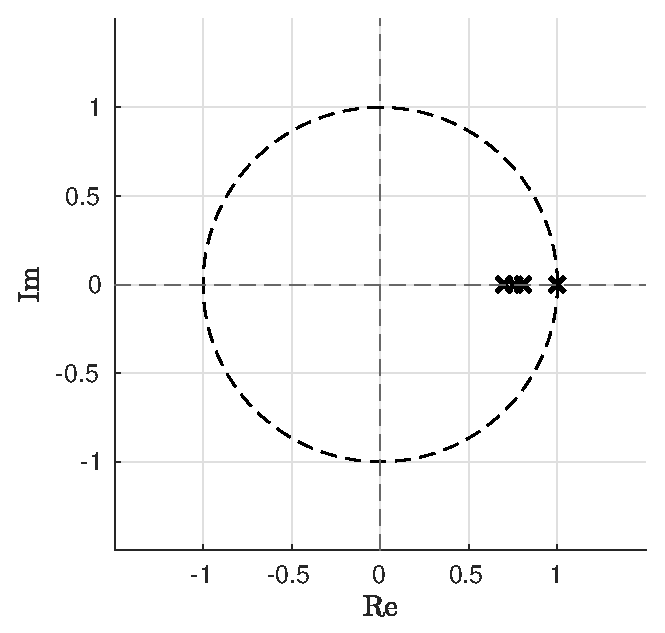
\includegraphics[height=3cm]{images/simulations/poles_simulations.eps}
    \end{subfigure}
    \hspace{0.3cm}
    \begin{subfigure}[b]{0.3\columnwidth}
        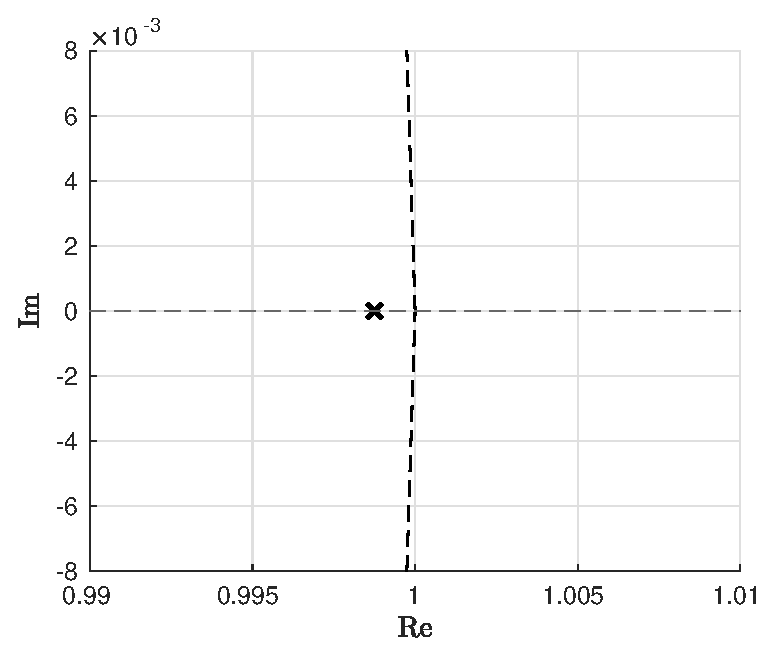
\includegraphics[height=3.2cm]{images/simulations/poles_simulations_zoom.eps}
    \end{subfigure}
    \caption{Poles of the closed-loop system in the imaginary plane}
    \label{fig:poles-simulation}
\end{figure}
% \textcolor{red}{change label for axes to X,Y. How to deal with 
% the legend?Use a star in all the plots for the desired position.}
Moving to the APFs, the mass of the Jetbot's robot is 
$M = \SI{1.4}{\kilo\gram}$ and it has been chosen $k_{Rep} = 700$
and $d_{Rep} = 5 \, R$.
In the simulations, the unicycles are treated as mass points but
nevertheless the objective is to verify if the physical robots will crash.
For this reason, the robots are considered to have collided in the simulation
if $d_{12} \leq 2 d_{Safe}$ (with $d_{Safe} = \SI{0.13}{\meter}$, 
see Fig.~\ref{fig:safety_distance}).
\begin{figure}
    \centering
    \vspace{-0.2cm}
    \hspace{1cm}
   \begin{subfigure}{0.3\columnwidth}
        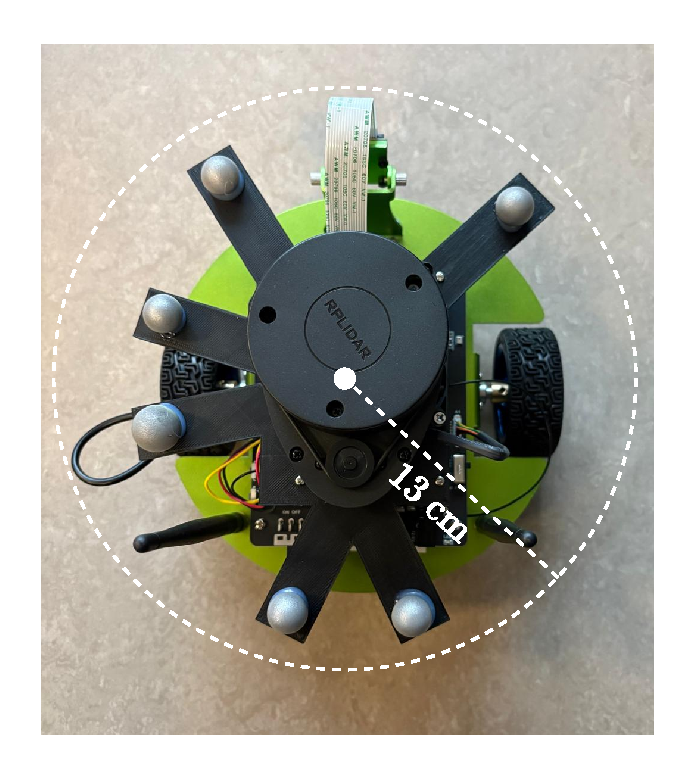
\includegraphics[height=3cm]{images/robot_dSafe.pdf}
    \end{subfigure}
    % \hspace{-0.6cm}
    \begin{subfigure}{0.3\columnwidth}
        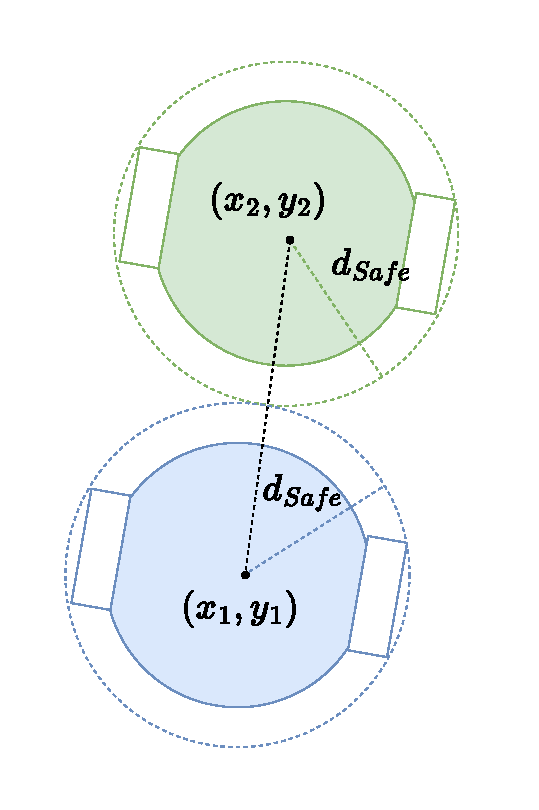
\includegraphics[height=3cm]{images/dSafe.pdf}
    \end{subfigure}
    \caption{The physical robot is contained entirely 
    in a circle of radius $d_{Safe} = \SI{0.13}{\meter}$.
    Consequently, if the centers of rotation are 
    at a distance less than $2d_{Safe}$
    it means that the agents collided.}
    \label{fig:safety_distance}
\end{figure}
For a quantitative analysis, the time required for the agents to reach 
the formation was studied.
Let us define the key performance index $\bar{t}$ as follows:
\begin{equation}
    \forall t \geq \bar{t}\ : \
    \left\{\begin{aligned}
        \left\lvert {e}_{A,x}(t) \right\rvert < \varepsilon &, \left\lvert {e}_{A,y}(t) \right\rvert < \varepsilon \\
        \left\lvert e_{\Delta_{A1,x}}(t) \right\rvert < \varepsilon &, \left\lvert e_{\Delta_{A1,y}}(t)\right\rvert < \varepsilon \\
        \left\lvert e_{\Delta_{12,x}}(t) \right\rvert < \varepsilon &, \left\lvert e_{\Delta_{12,y}}(t) \right\rvert < \varepsilon \\
    \end{aligned} \right.
\end{equation}
with $\varepsilon$ a negligible error. For the simulations, it has been set 
$\varepsilon = \SI{0.10}{\meter}$.

The first set of simulations considers a scenario with the ground clean 
and without disturbances, i.e. $\boldsymbol{d}(k) = 0$.
The results are shown in Fig.~\ref{fig:sim_withAPF_noNoise}.
For each unicycle, they are plotted the 2D-trajectories 
of the center of rotation and of the point $(x_{R_i}, y_{R_i})$ 
with a solid and a dotted line respectively.
The desired inter distances drone-$G_1$ and $G_1$-$G_2$ are plotted 
with solid black, while the actual inter distances at the end of the simulation 
are the dotted black lines.
Finally, stars denote the desired final positions of the robots 
based on the definitions of $(x^d_A, y^d_A)$, $ \Delta^d_{A1}$ and $\Delta^d_{12}$.
\begin{figure}
    \centering
    \begin{subfigure}[b]{0.32\columnwidth}
        \centering
        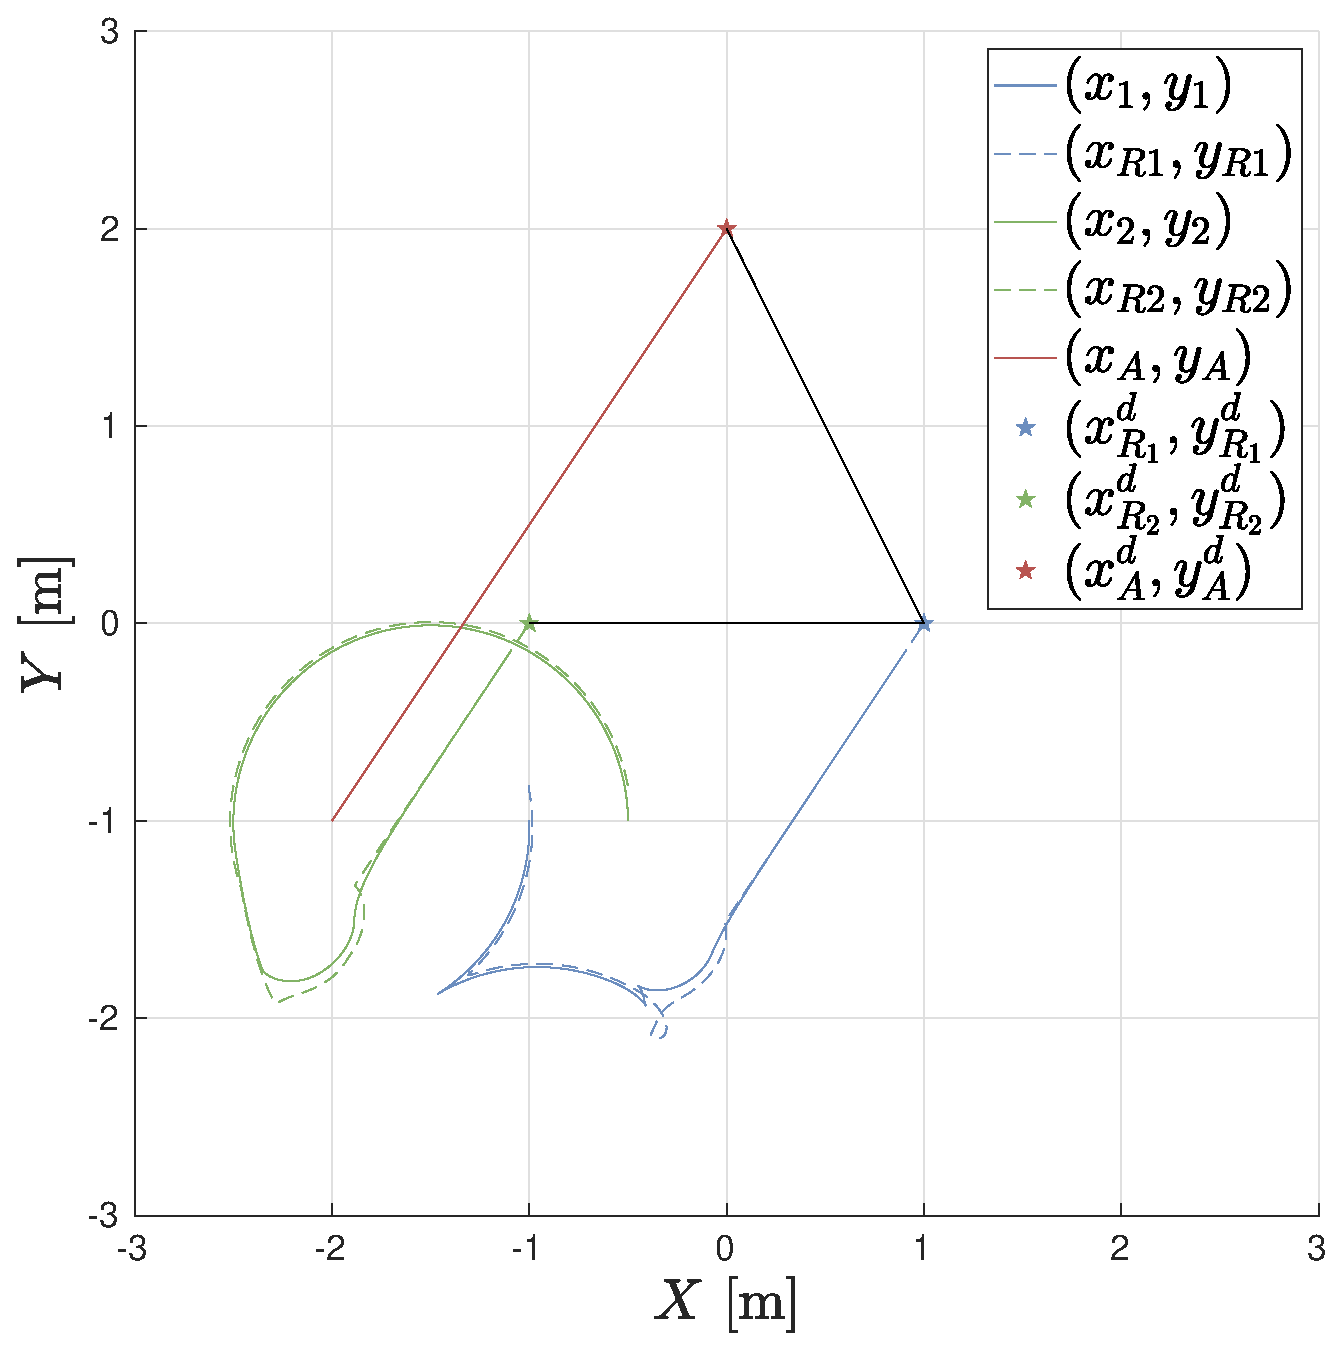
\includegraphics[width=\linewidth]{images/simulations/with_APF/not_noisy/1st_scenario_with_noNoise.eps}
         \caption{Triangle Top}
         \label{fig:sim_withAPF_noNoise_1}
    \end{subfigure}
    \begin{subfigure}[b]{0.32\columnwidth}
        \centering
        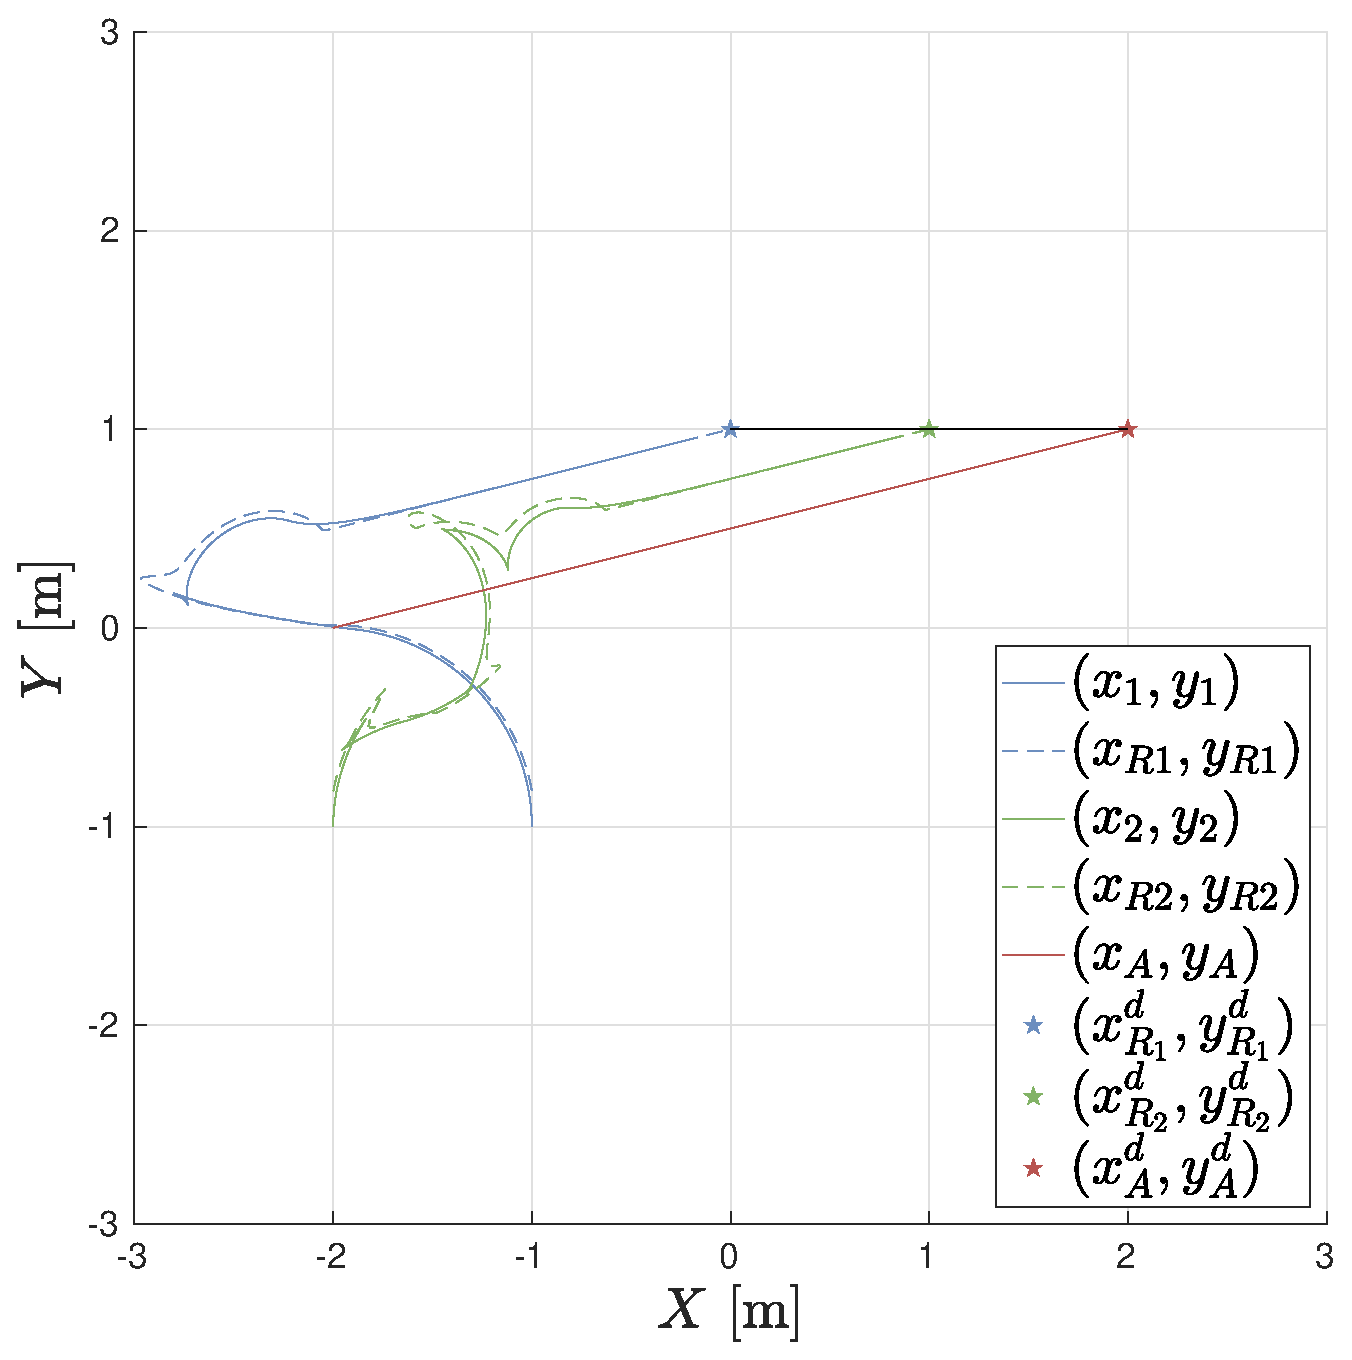
\includegraphics[width=\linewidth]{images/simulations/with_APF/not_noisy/2nd_scenario_with_noNoise.eps}
        \caption{Line Segment}
         \label{fig:sim_withAPF_noNoise_2}
    \end{subfigure}
    \begin{subfigure}[b]{0.32\columnwidth}
        \centering
        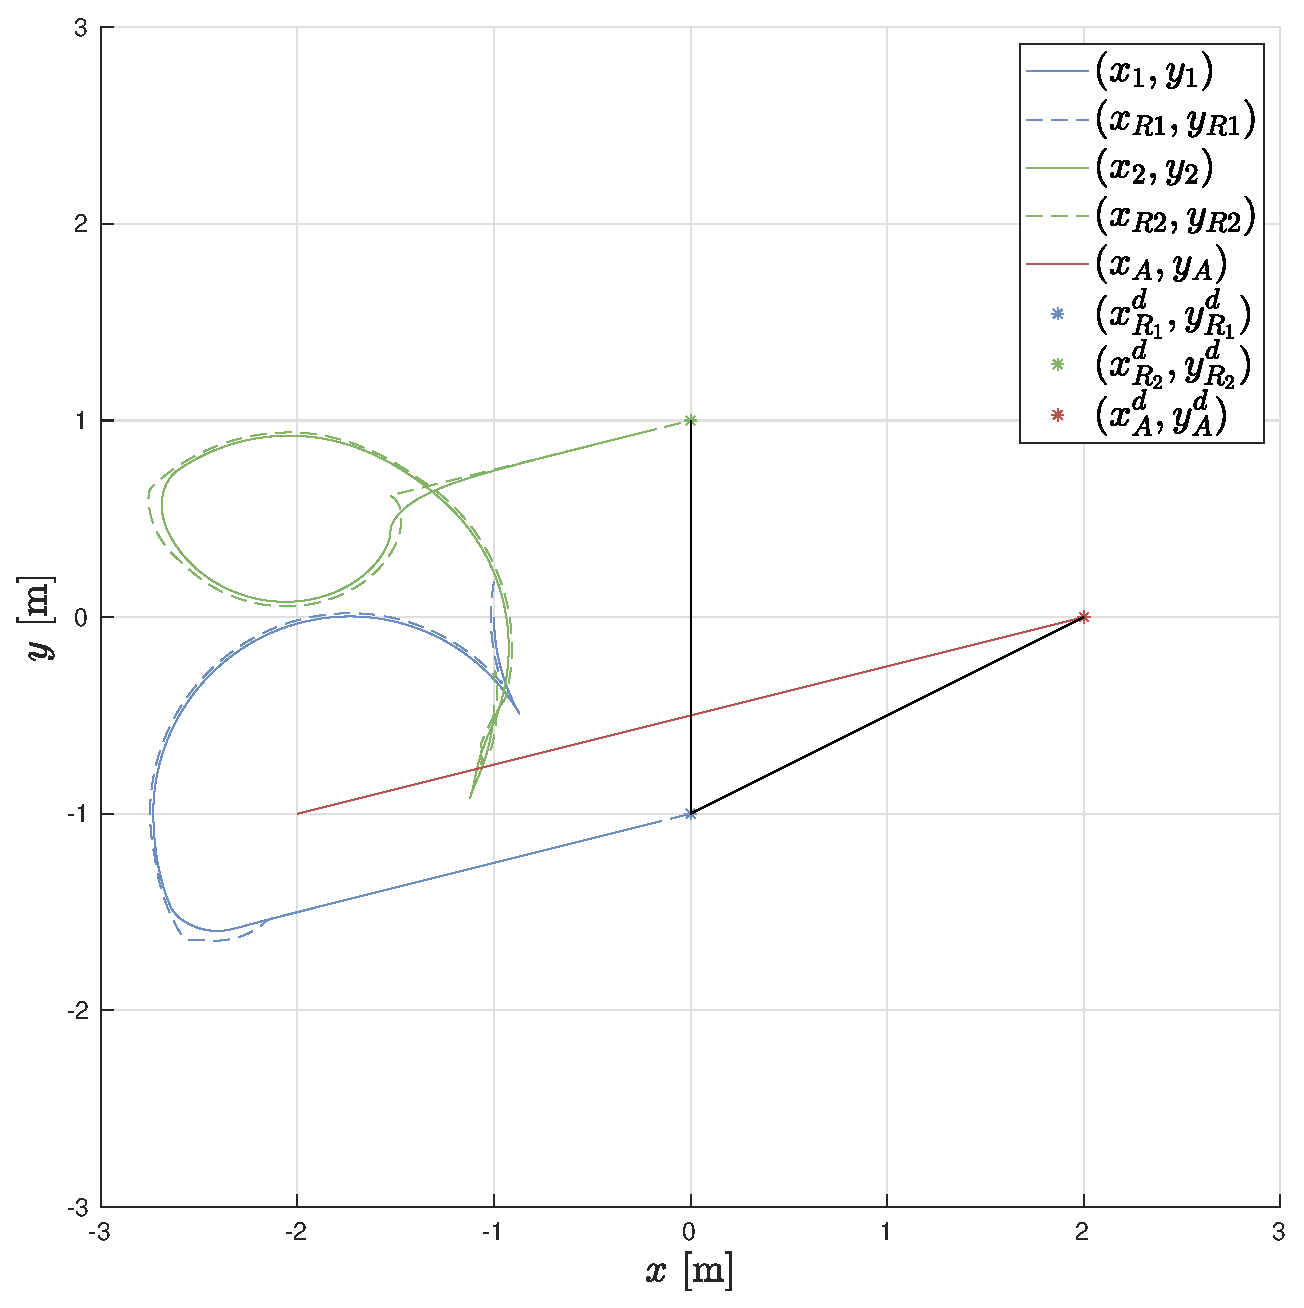
\includegraphics[width=\linewidth]{images/simulations/with_APF/not_noisy/3rd_scenario_with_noNoise.eps}
      \caption{Triangle Right}
         \label{fig:sim_withAPF_noNoise_3}
    \end{subfigure}
    \vspace{-0.2cm}
    \caption{Trajectories of the three agents with desired and actual interdistances in ideal simulations.}
    \label{fig:sim_withAPF_noNoise}
\end{figure}
From Fig.~\ref{fig:sim_withAPF_noNoise}, it is straightforward to conclude that the agents make the formation avoiding collisions in 
all scenarios, which differ in initial conditions and desired geometric shapes.
The key performance index for the first scenario is $\bar{t} = \SI{54.76}{\second}$,
for the second case $\bar{t} = \SI{59.38}{\second}$, and for 
the last case $\bar{t} = \SI{59.38}{\second}$.

To demonstrate the importance of APFs, the simulations have been redone without repulsive
forces.
If a collision occurs this time, the ground vehicles will halt and remain stopped until 
the end of the test.
Fig.~\ref{fig:sim_woAPF_noNoise} displays the resulting trajectories.
\begin{figure}
    \centering
    \begin{subfigure}[b]{0.32\columnwidth}
        \centering
        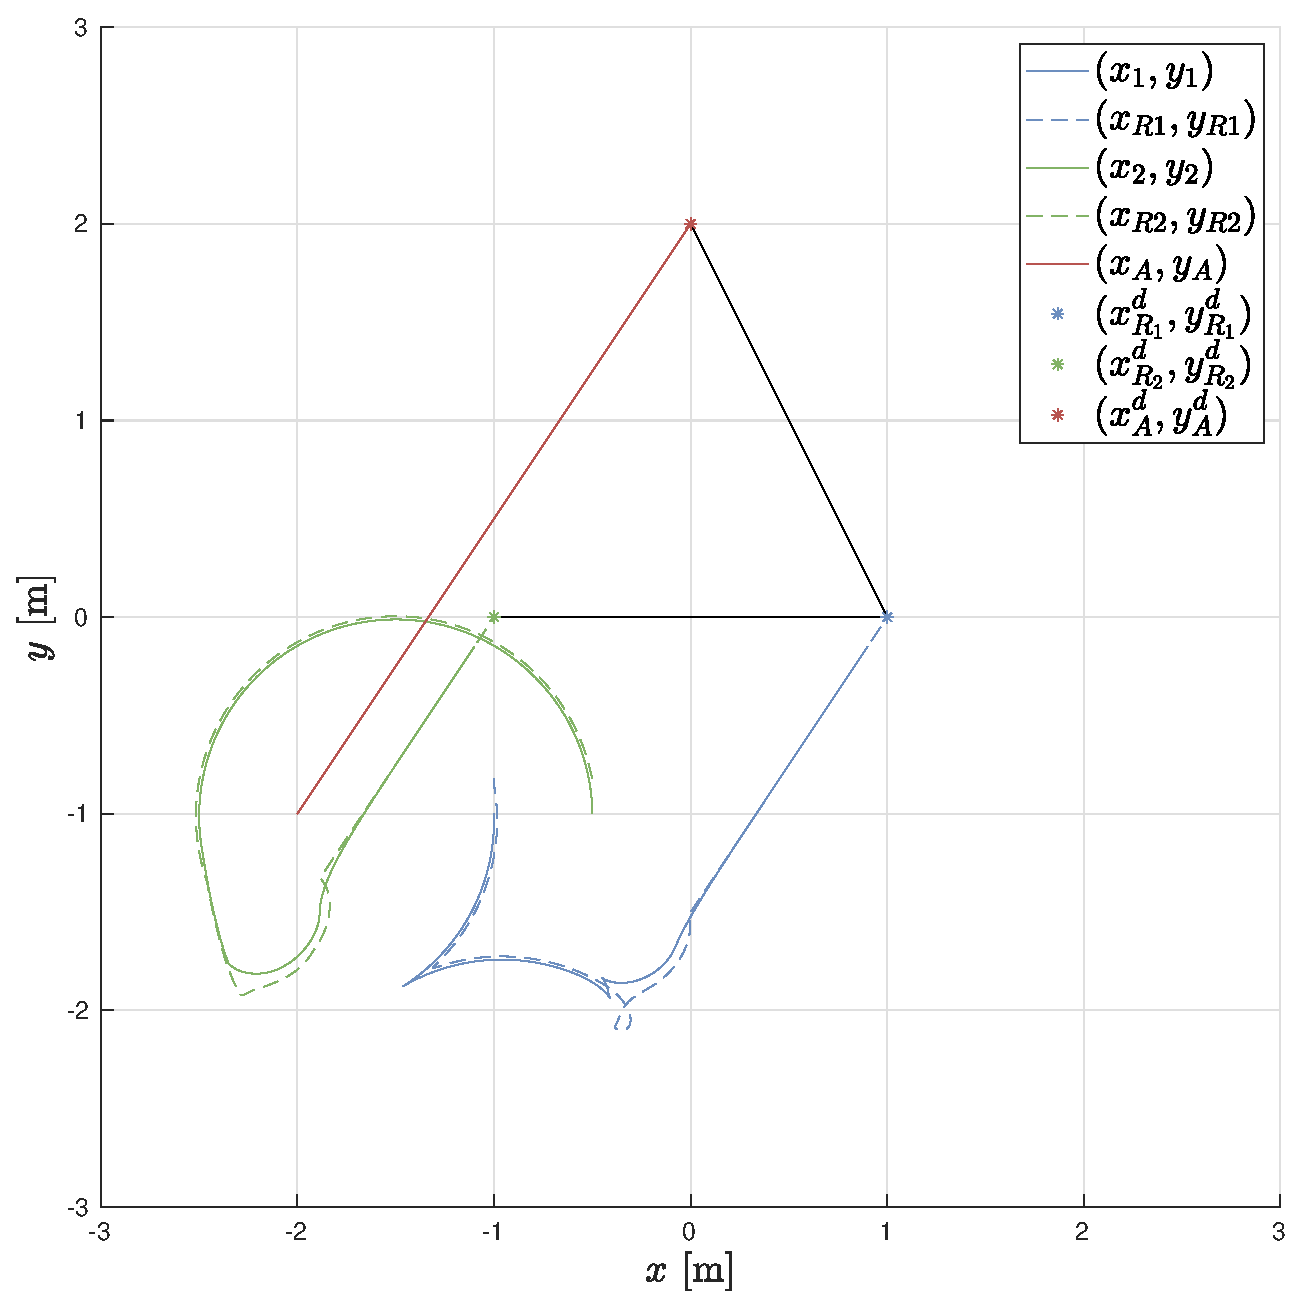
\includegraphics[width=\linewidth]{images/simulations/wo_APF/1st_scenario_wo.eps}
        \caption{Triangle Top}
        \label{fig:sim_woAPF_noNoise_1}
    \end{subfigure}
    \begin{subfigure}[b]{0.32\columnwidth}
        \centering
        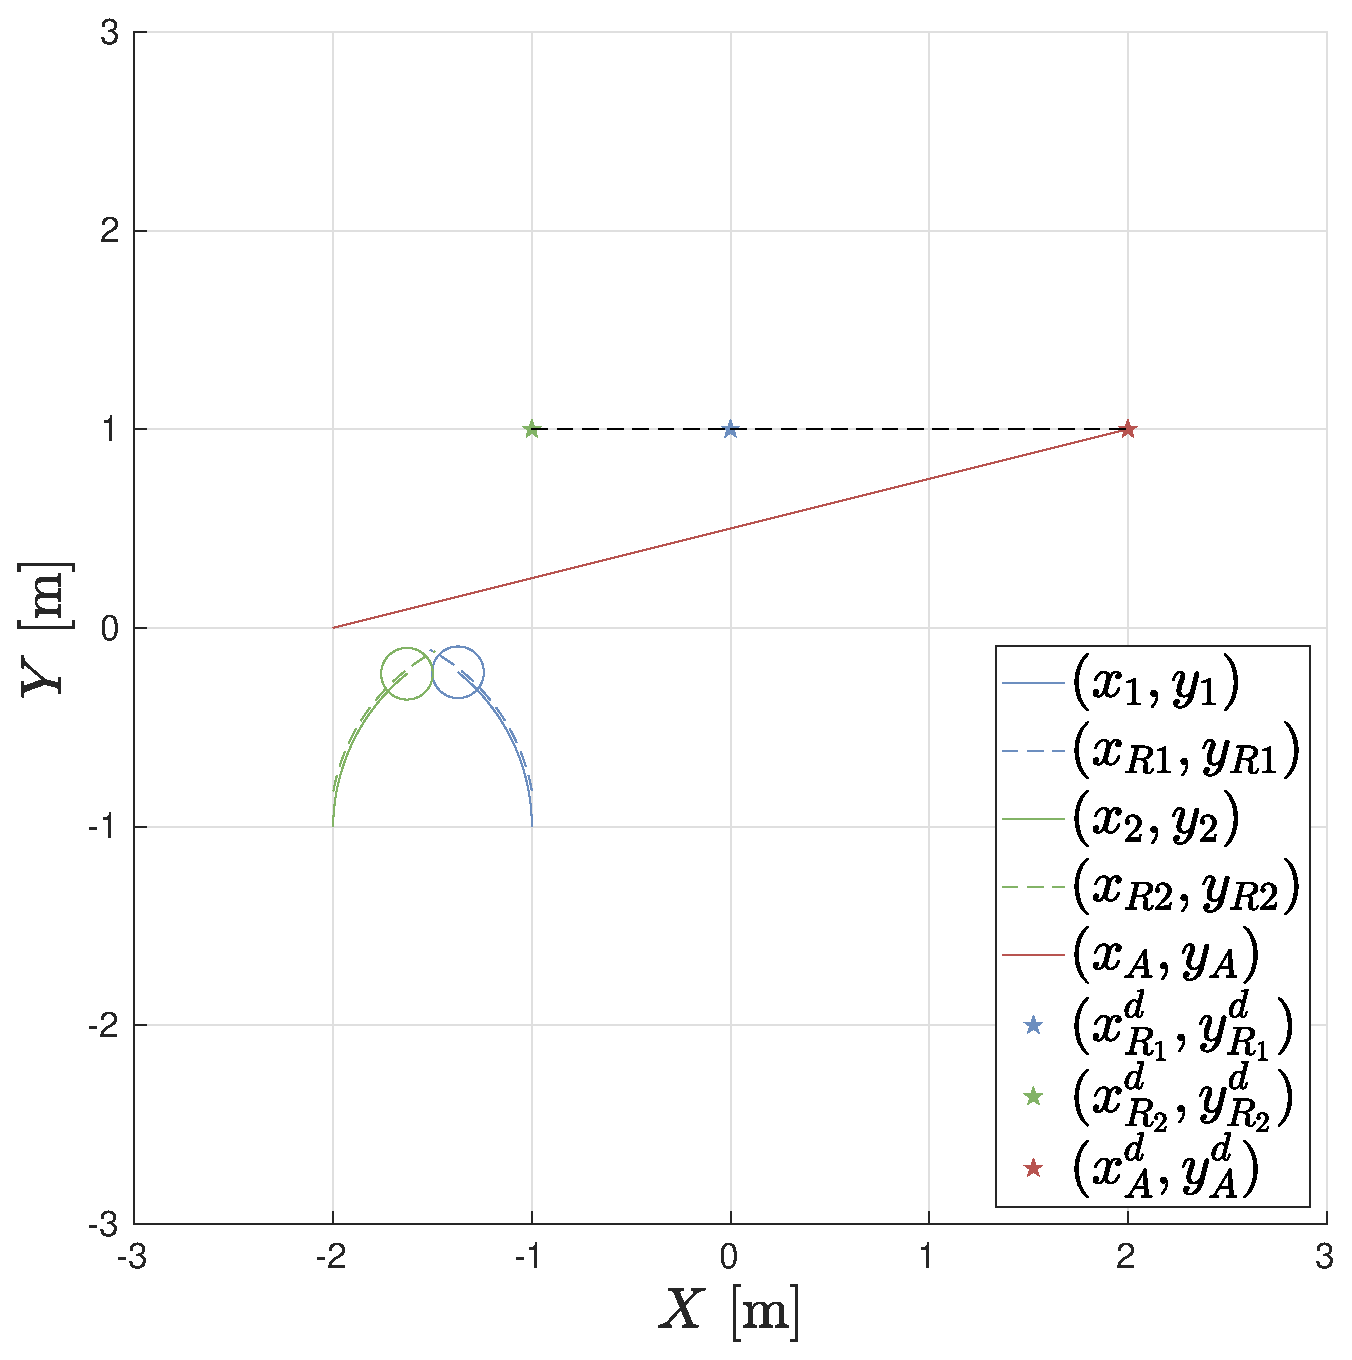
\includegraphics[width=\linewidth]{images/simulations/wo_APF/2nd_scenario_wo.eps}
        \caption{Line Segment}
         \label{fig:sim_woAPF_noNoise_2}
    \end{subfigure}
    % \hfill
    \begin{subfigure}[b]{0.32\columnwidth}
        \centering
        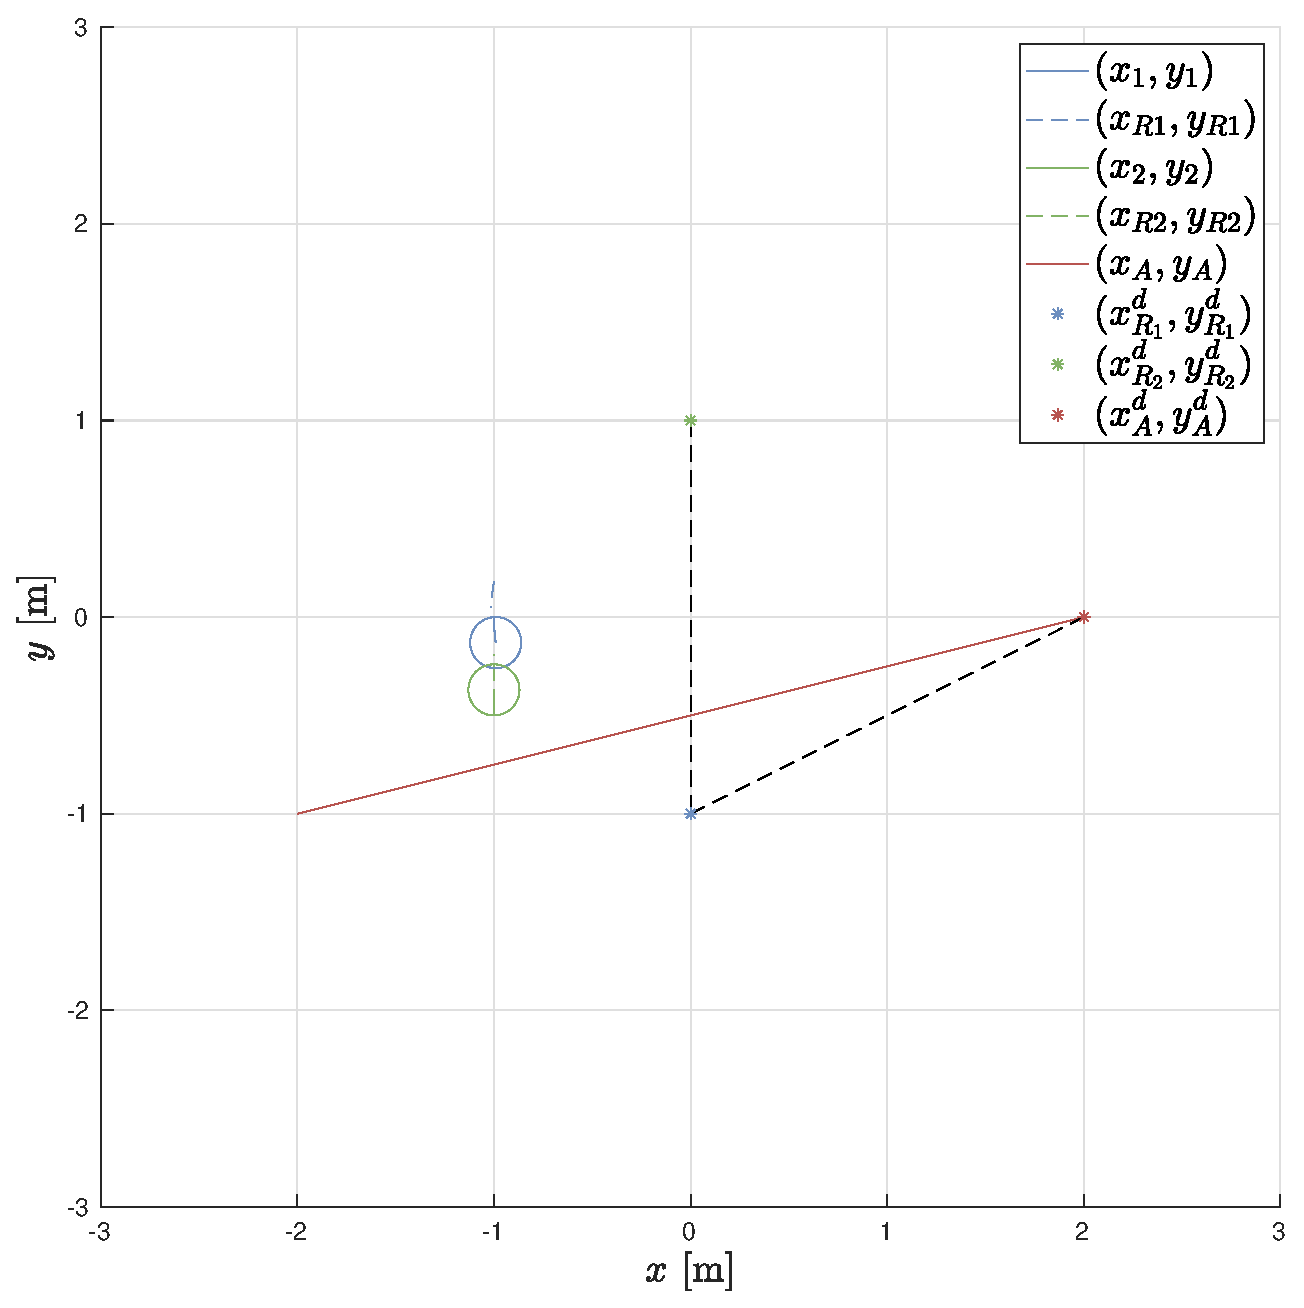
\includegraphics[width=\linewidth]{images/simulations/wo_APF/3rd_scenario_wo.eps}
        \caption{Triangle Right}
         \label{fig:sim_woAPF_noNoise_3}
    \end{subfigure}
    \vspace{-0.2cm}
    \caption{Trajectories of the three agents without APF in ideal simulations.}
    \label{fig:sim_woAPF_noNoise}
\end{figure}
In the first case, the curves are the same as Fig.~\ref{fig:sim_withAPF_noNoise_1} since 
the unicycles do not clash.
However, the differences are obvious in the other two cases: compare
Fig.~\ref{fig:sim_woAPF_noNoise_2} and Fig.~\ref{fig:sim_woAPF_noNoise_3} with
Fig.~\ref{fig:sim_withAPF_noNoise_2} and Fig.~\ref{fig:sim_withAPF_noNoise_3}.
It is clear  that without APF, the unicycles get too close and they must stop.
Hence, even if the drone reaches the desired position $(x^d_A, y^d_A)$, 
the overall formation is not attained by the fleet.
On the opposite, thanks to the artificial repulsive forces the robot $G_2$ 
deviates its path to stay at a safe distance from $G_1$.


The last set of simulations aims to study the robustness of the proposed control 
scheme in the presence of the zero-mean disturbance $\boldsymbol{d}(k)$.
The disturbance has been modeled in particular 
as a gaussian noise with variance $\Sigma = 0.1 I_{6\times6}$.
The results are presented in Fig.~\ref{fig:sim_withAPF_noisy}.
\begin{figure}
    \centering
    \begin{subfigure}[b]{0.32\columnwidth}
        \centering
        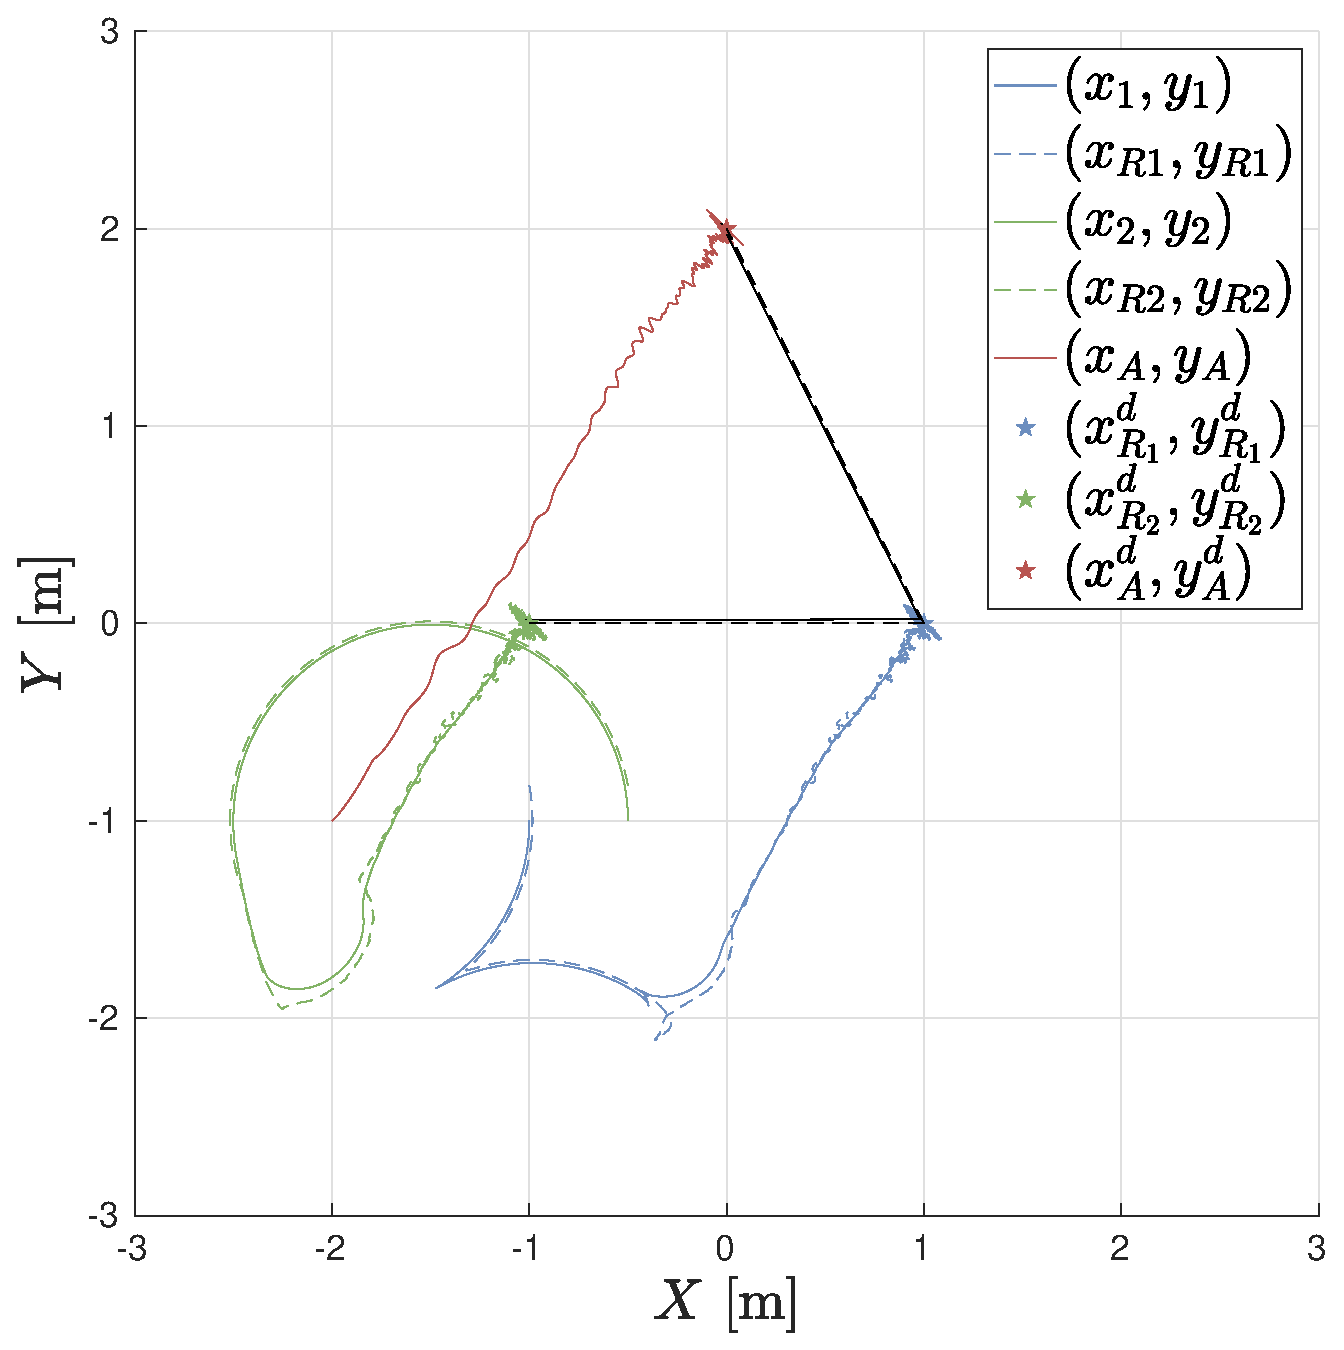
\includegraphics[width=\linewidth]{images/simulations/with_APF/noisy/1st_scenario_with_noisy.eps}
         \caption{Triangle Top}
    \end{subfigure}
    \begin{subfigure}[b]{0.32\columnwidth}
        \centering
        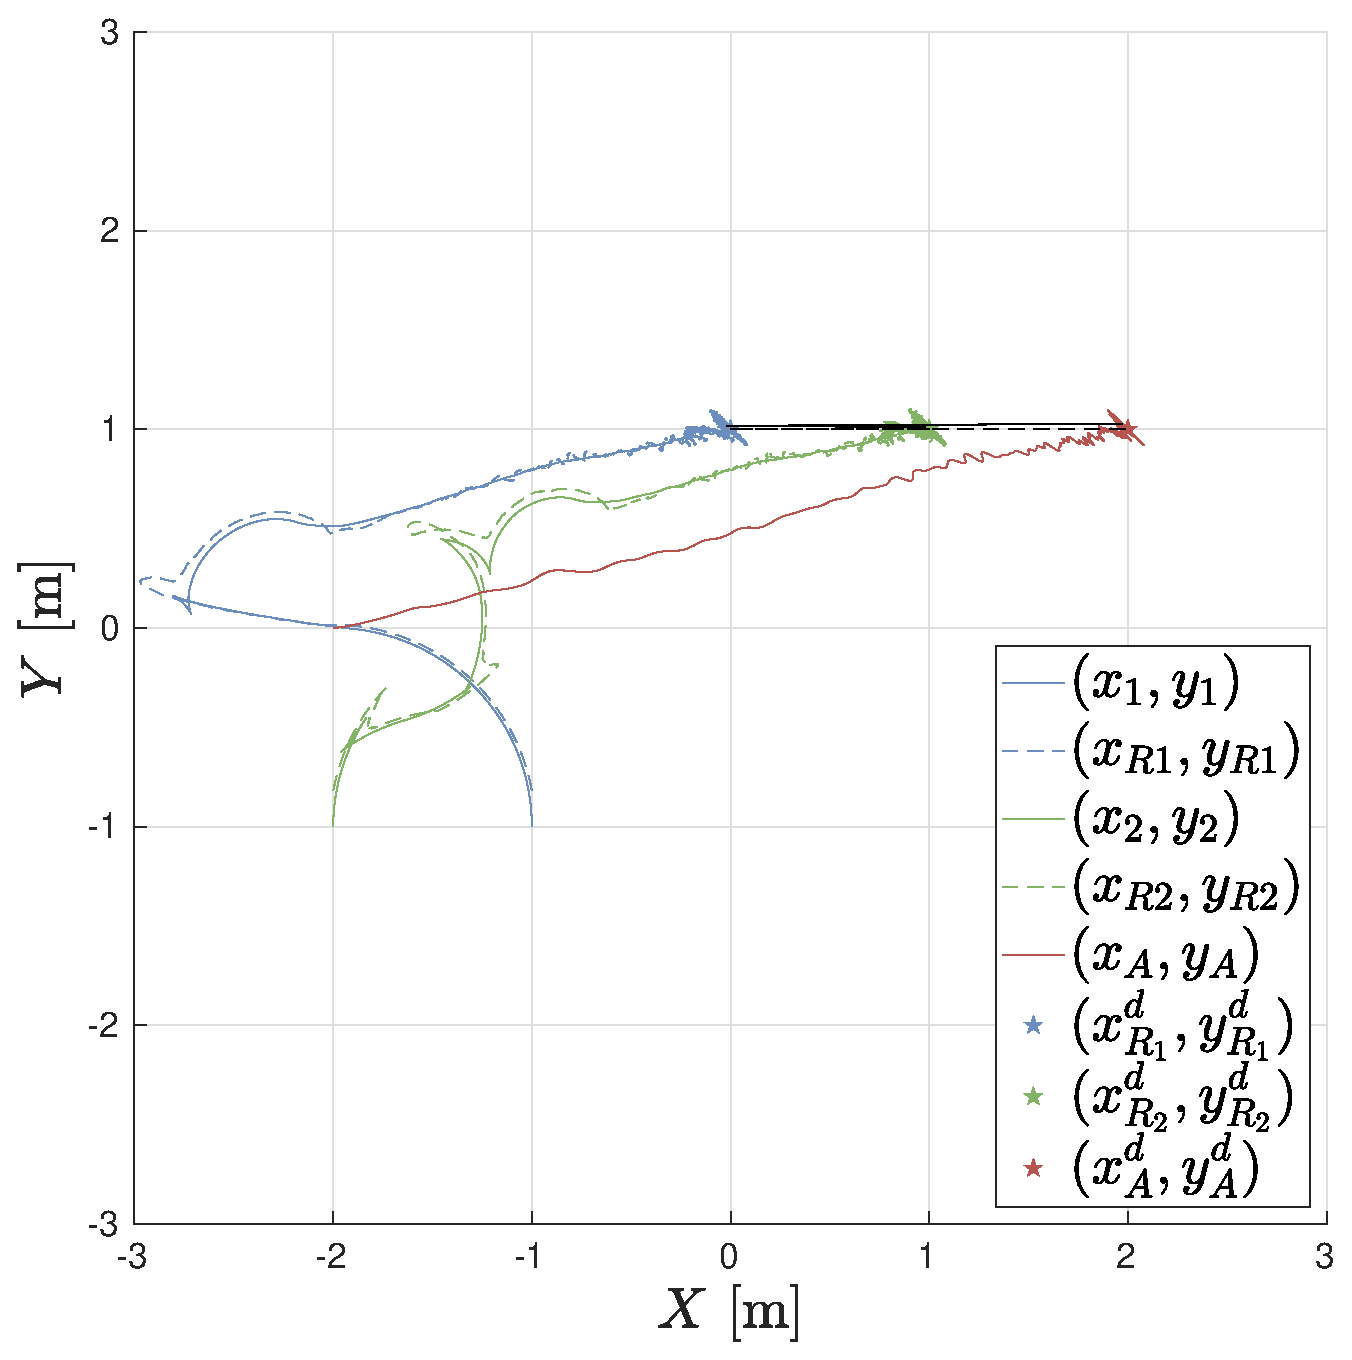
\includegraphics[width=\linewidth]{images/simulations/with_APF/noisy/2nd_scenario_with_noisy.eps}
        \caption{Line Segment}
    \end{subfigure}
    \begin{subfigure}[b]{0.32\columnwidth}
        \centering
        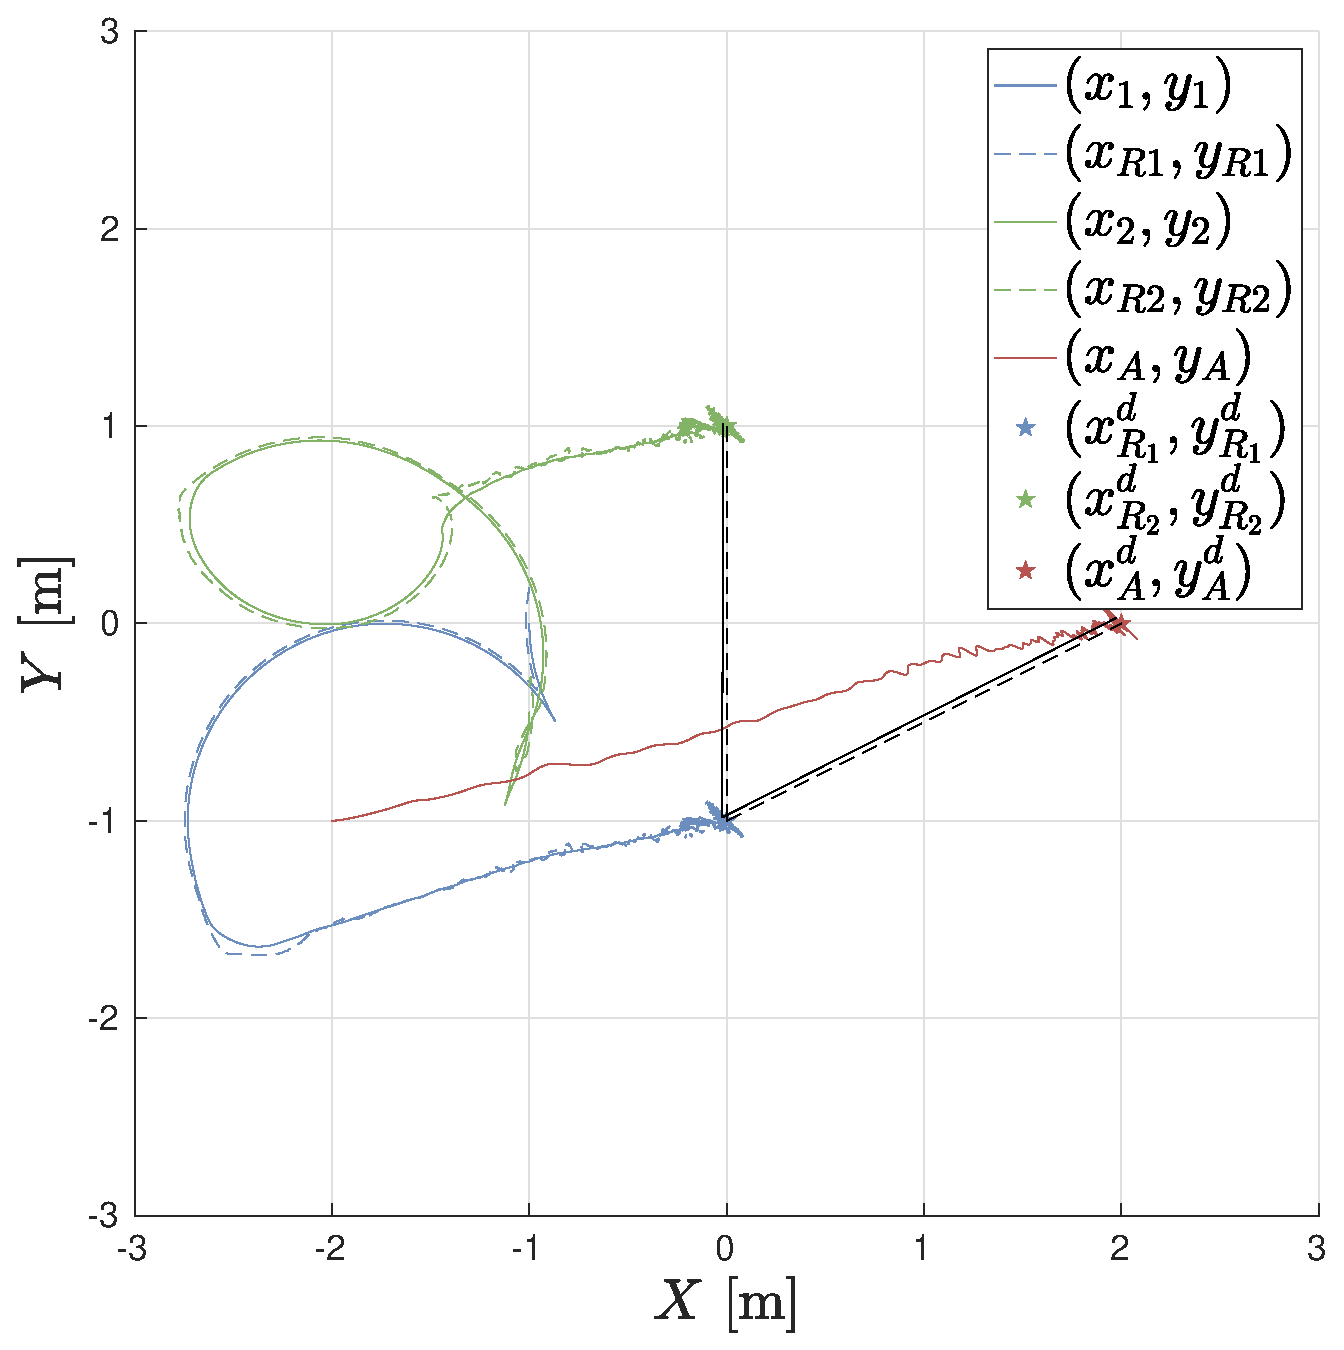
\includegraphics[width=\linewidth]{images/simulations/with_APF/noisy/3rd_scenario_with_noisy.eps}
      \caption{Triangle Right}
    \end{subfigure}
    \vspace{-0.2cm}
    \caption{Trajectories of the three agents with desired and actual interdistances in simulation with disturbances.}
    \label{fig:sim_withAPF_noisy}
\end{figure}
The trajectories are similar to the ones in Fig.~\ref{fig:sim_withAPF_noNoise},
but the agents in the end oscillate around the desired final positions due to disturbance $\boldsymbol{d}(k)$
(though they remain within a small neighborhood).
This is the same reason why the solid and dotted lines do not exactly overlap:
the dotted shape appears to be a translated version of the solid one.
However, collisons between $G_1$ and $G_2$ are avoided and the formation is reached after
$\bar{t} = \SI{54.22}{\second}$, $\bar{t} = \SI{112.14}{\second}$, and 
$\bar{t} = \SI{112.1}{\second}$ respectively.





\section{Experimental Validation}
\label{sec:experimental_validation}
\textcolor{red}{dire che usi FL-AIR per il drone, pensa 
se incrementare $\varepsilon$ a 20cm invece di 17cm e rifare 
i plot come nelle simulazioni (stelle e XY)}
\begin{figure}
    \centering
    \begin{subfigure}[b]{0.31\columnwidth}
        \centering
        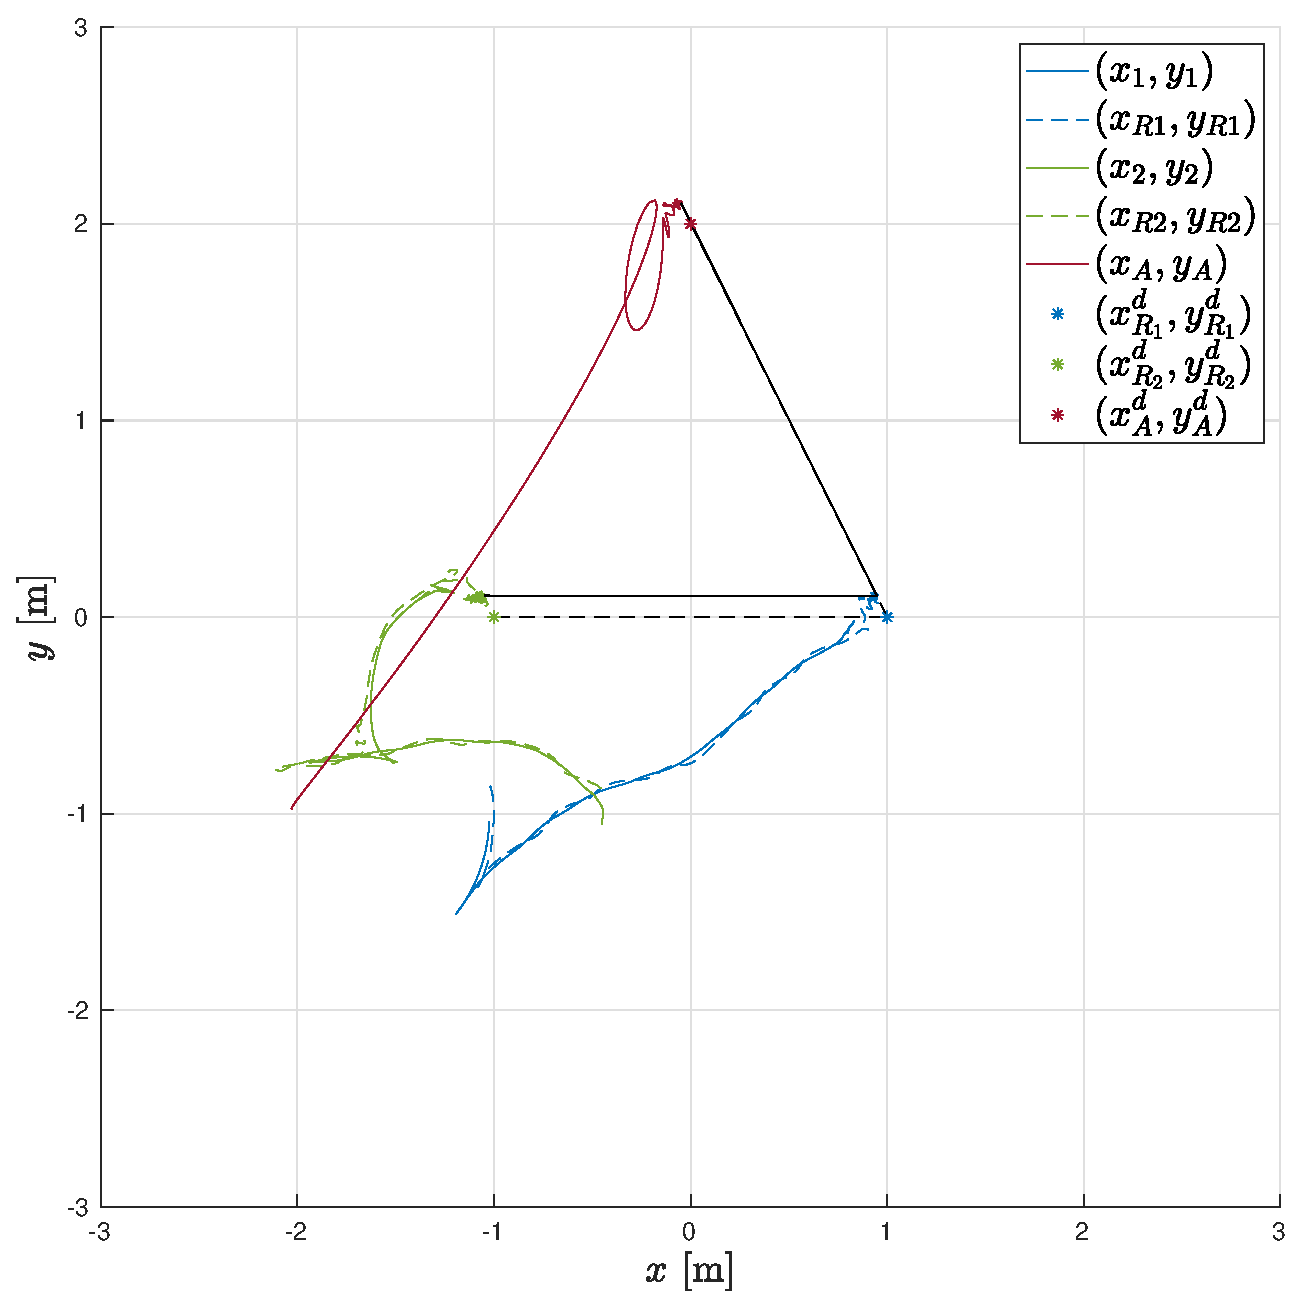
\includegraphics[width=\linewidth]{images/experiment/nominal/1st_scenario_exp.eps}
        \caption{Triangle Top}
    \end{subfigure}
    \begin{subfigure}[b]{0.31\columnwidth}
        \centering
        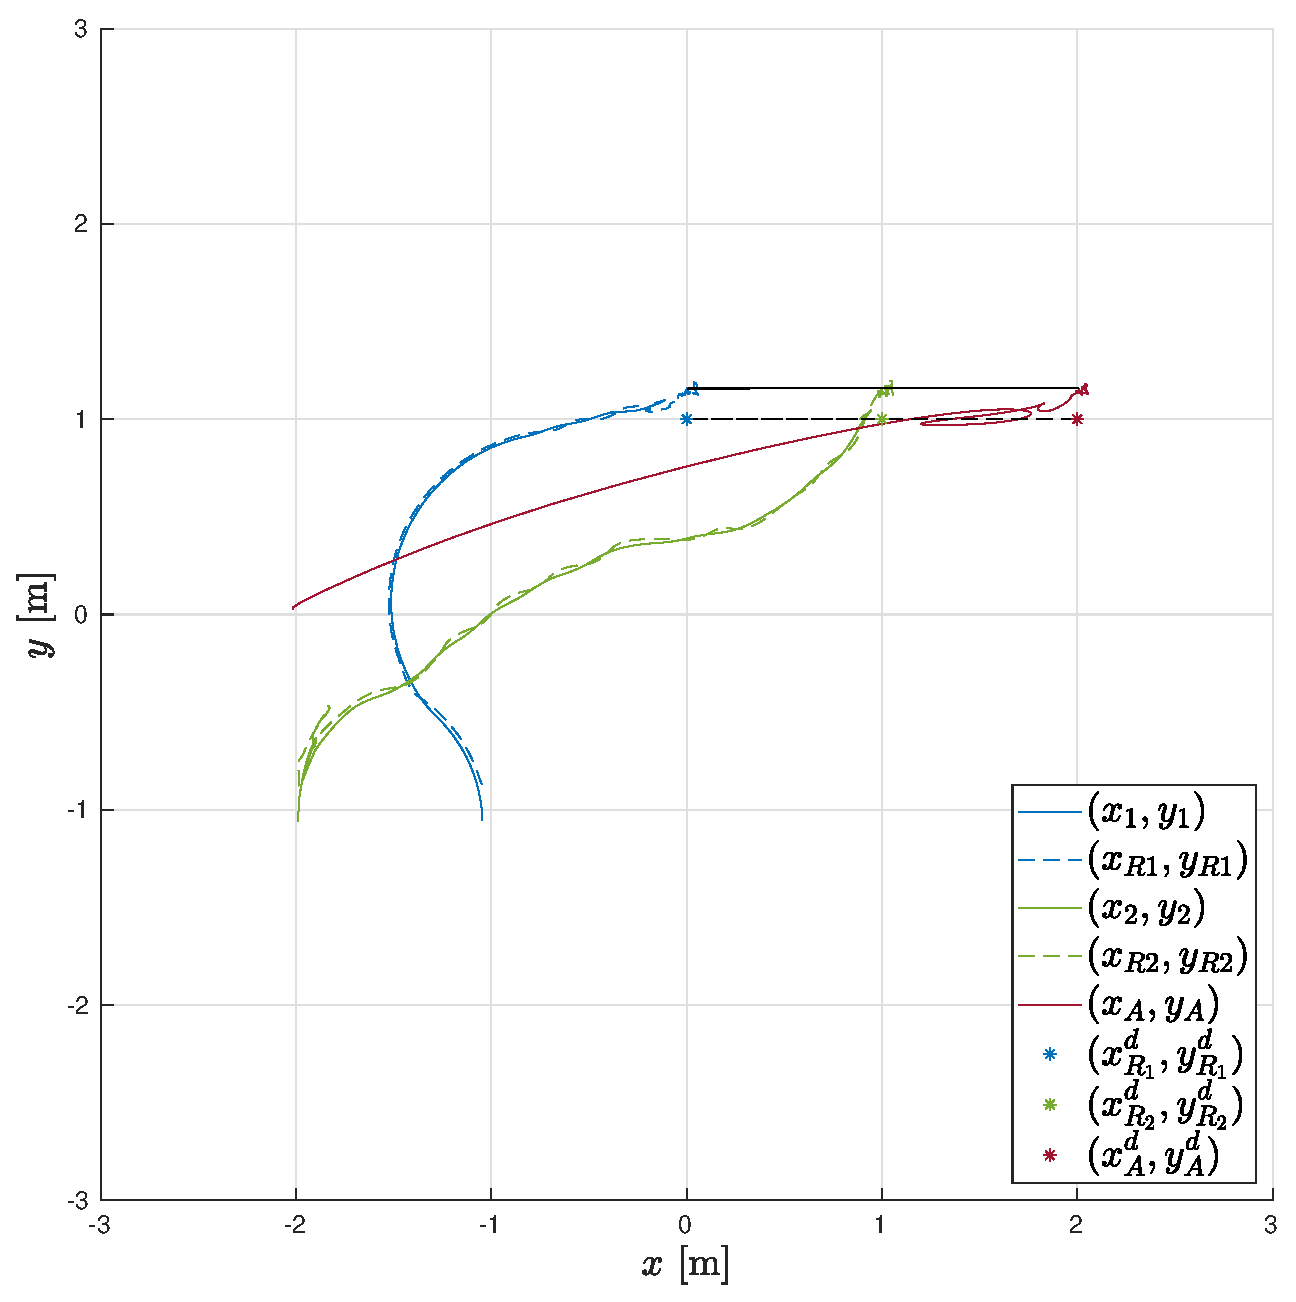
\includegraphics[width=\linewidth]{images/experiment/nominal/2nd_scenario_exp.eps}
      \caption{Line Segment}
   \end{subfigure}
    \begin{subfigure}[b]{0.31\columnwidth}
        \centering
        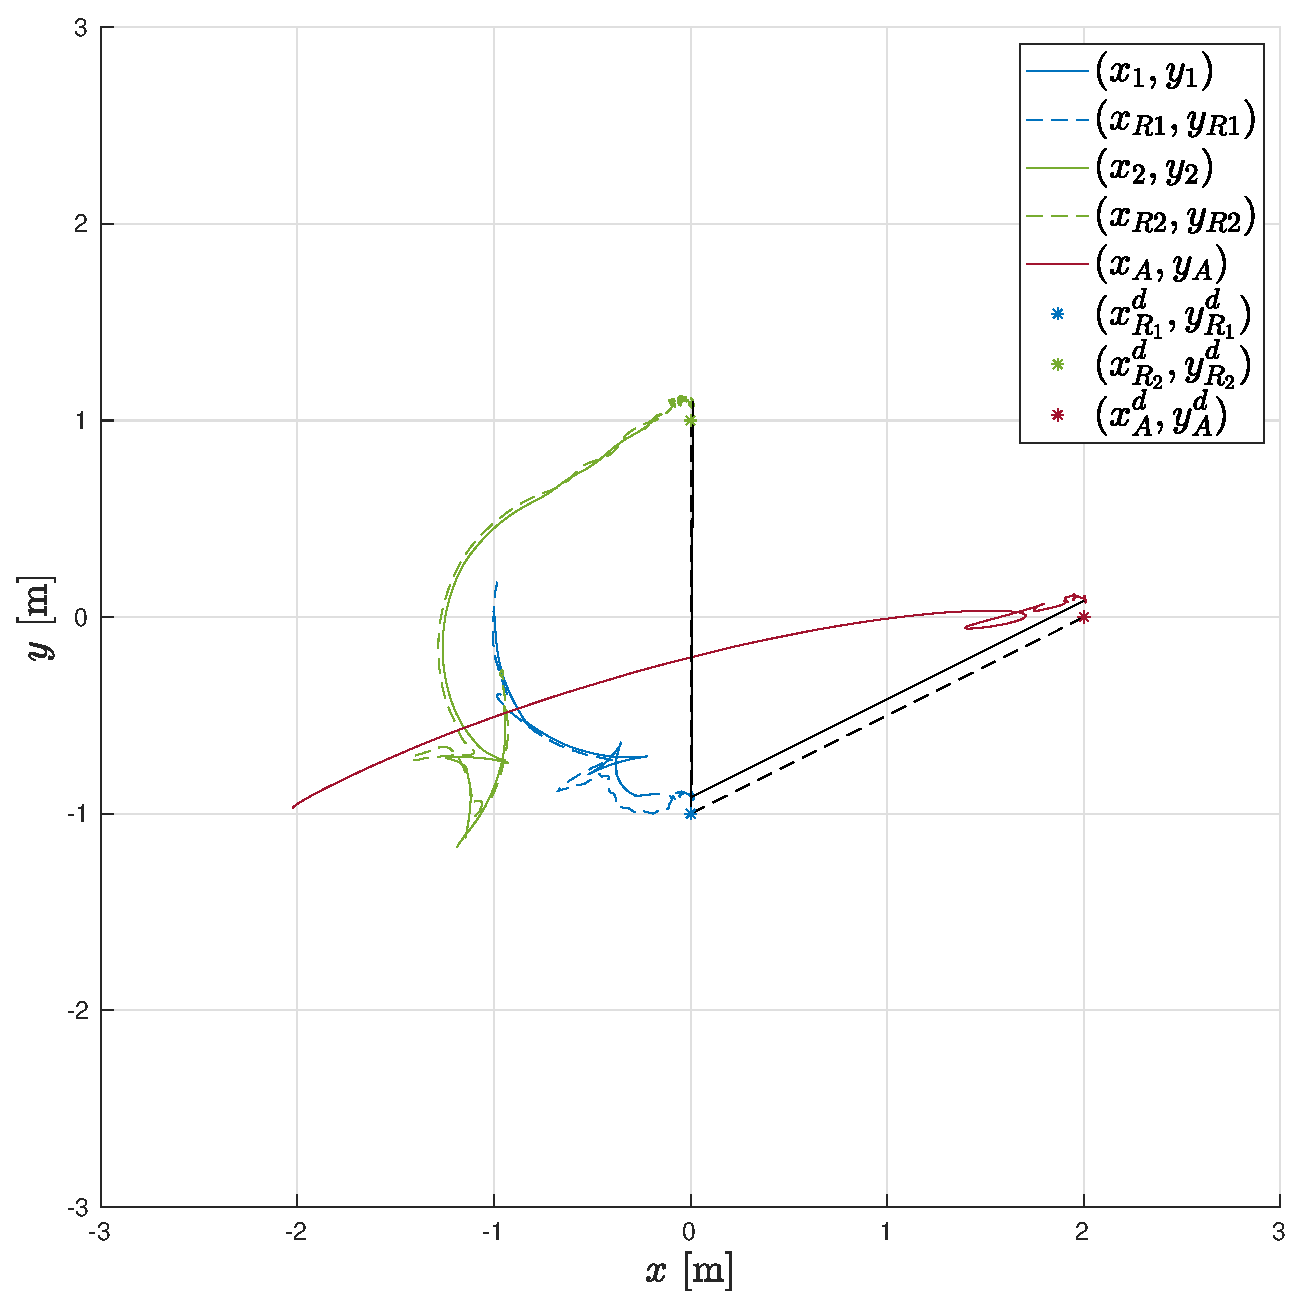
\includegraphics[width=\linewidth]{images/experiment/nominal/3rd_scenario_exp.eps}
        \caption{Triangle Right}
      \end{subfigure}
   \vspace{-0.2cm}
   \caption{Trajectories of the three agents with desired and actual interdistances in the experiments.}
\end{figure}

For each obstacle, just add a corrective APF term: \textcolor{red}{add formula}

Increased $y_A^d$ of $\SI{0.5}{\meter}$, 
formation reached after \SI{55.30}{\second}(the drone 
takes some time, but $R_2$ achieve the formation w.r.t 
$R_1$ after \SI{16.02}{\second}), when swapped
the formation is achieved after \SI{9.74}{\second} 
(drone after \SI{8.32}{\second}
while $R_2$ after \SI{9.74}{\second}).


\begin{figure}[h!]
    \centering
    \begin{subfigure}[b]{0.31\columnwidth}
        \centering
        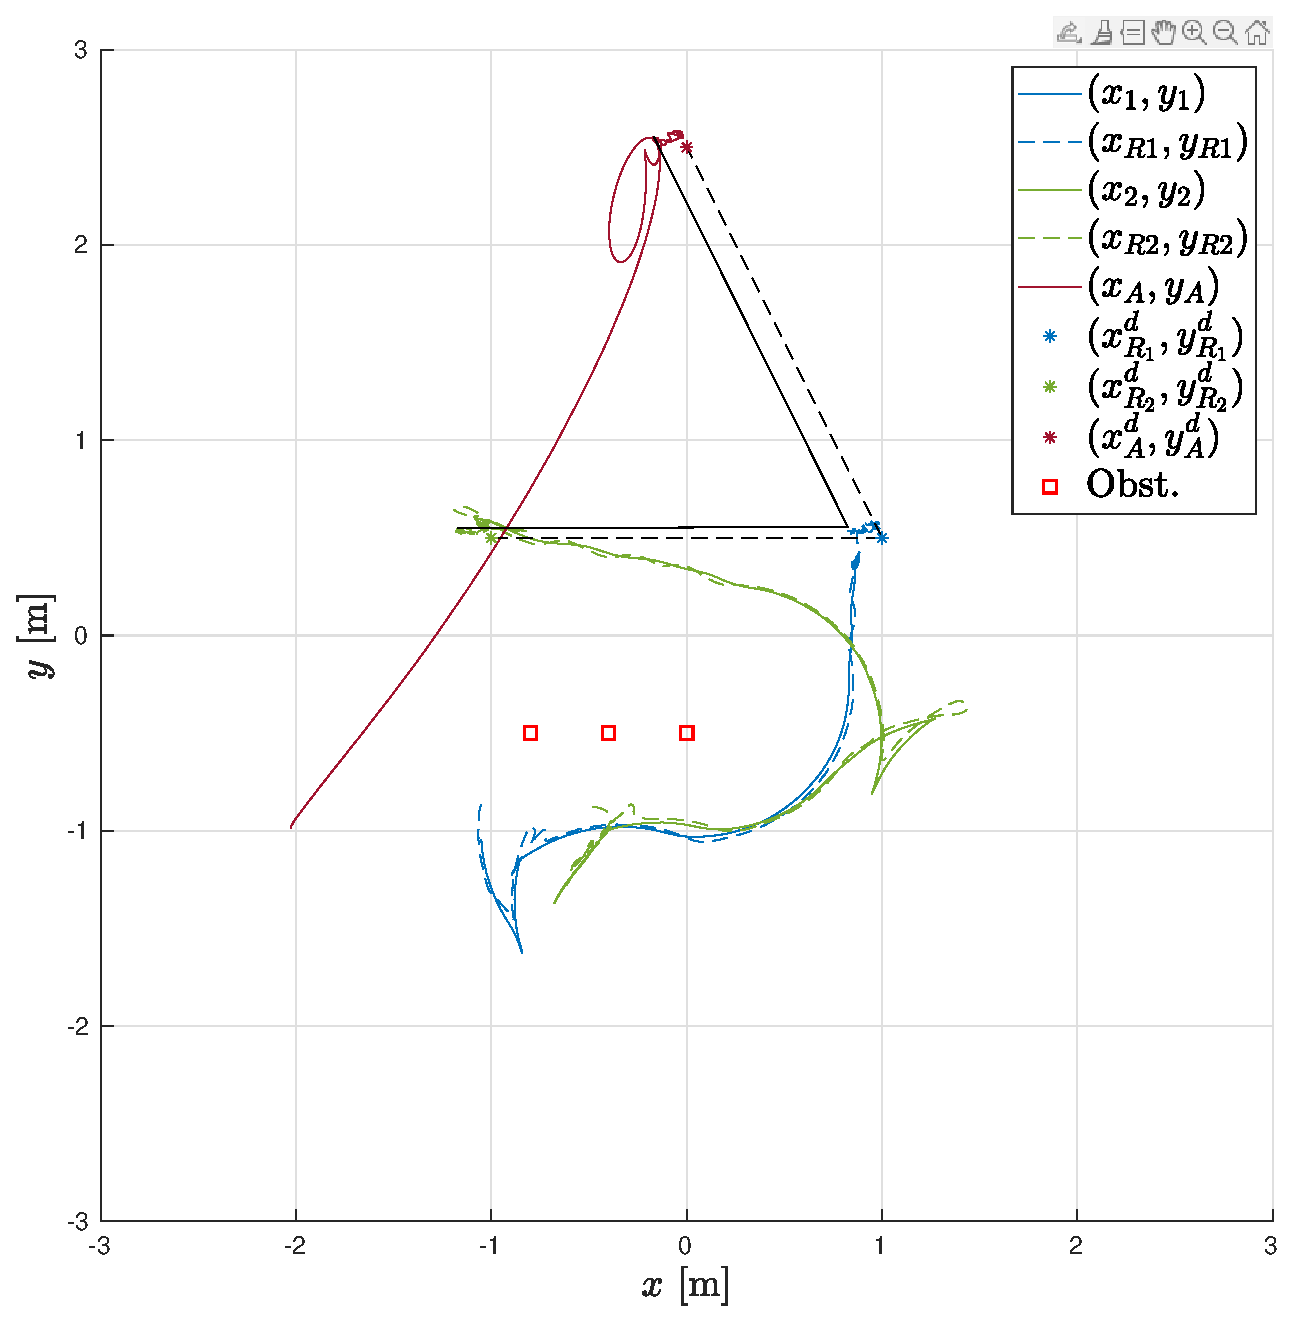
\includegraphics[width=\linewidth]{images/experiment/static_obstacles/1st_scenario_obs_exp.eps}
        \caption{$R_2$ on the right}
    \end{subfigure}
    \begin{subfigure}[b]{0.31\columnwidth}
        \centering
        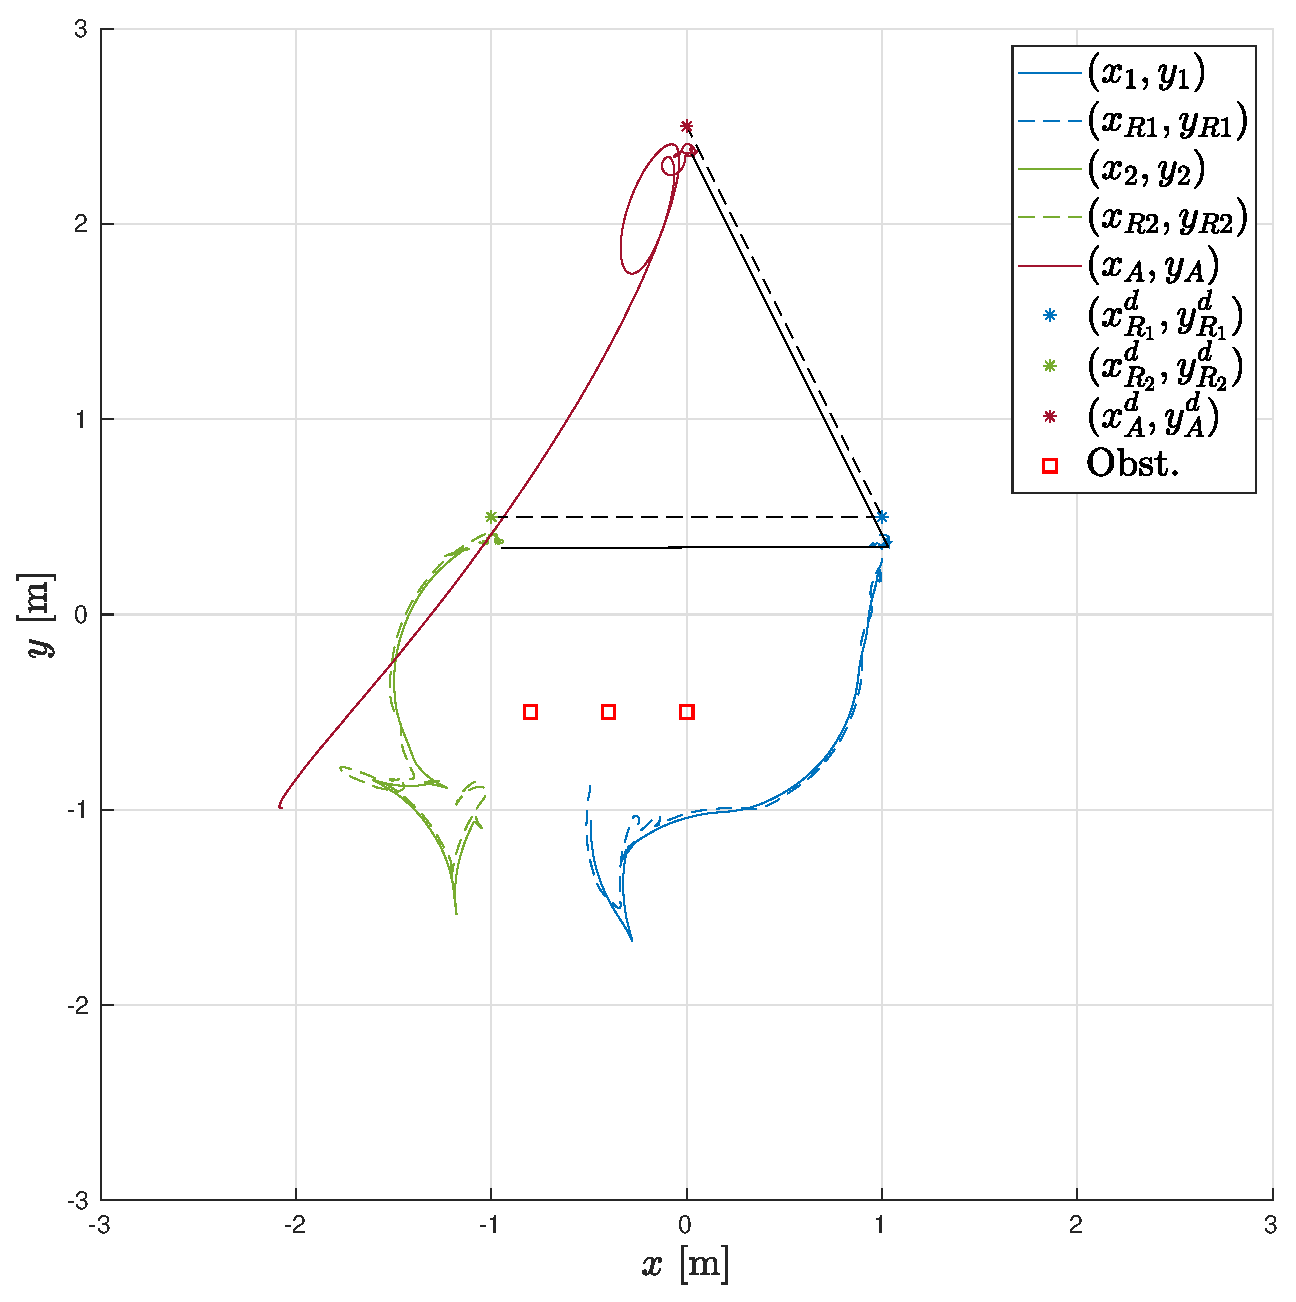
\includegraphics[width=\linewidth]{images/experiment/static_obstacles/1st_scenario_exp_obs_swap.eps}
        \caption{$R_2$ on the left}
    \end{subfigure}
    \vspace{-0.2cm}
    \caption{\textcolor{red}{TODO}}
\end{figure}


\begin{figure}
    \centering
    \begin{subfigure}[b]{0.32\columnwidth}
        \centering
        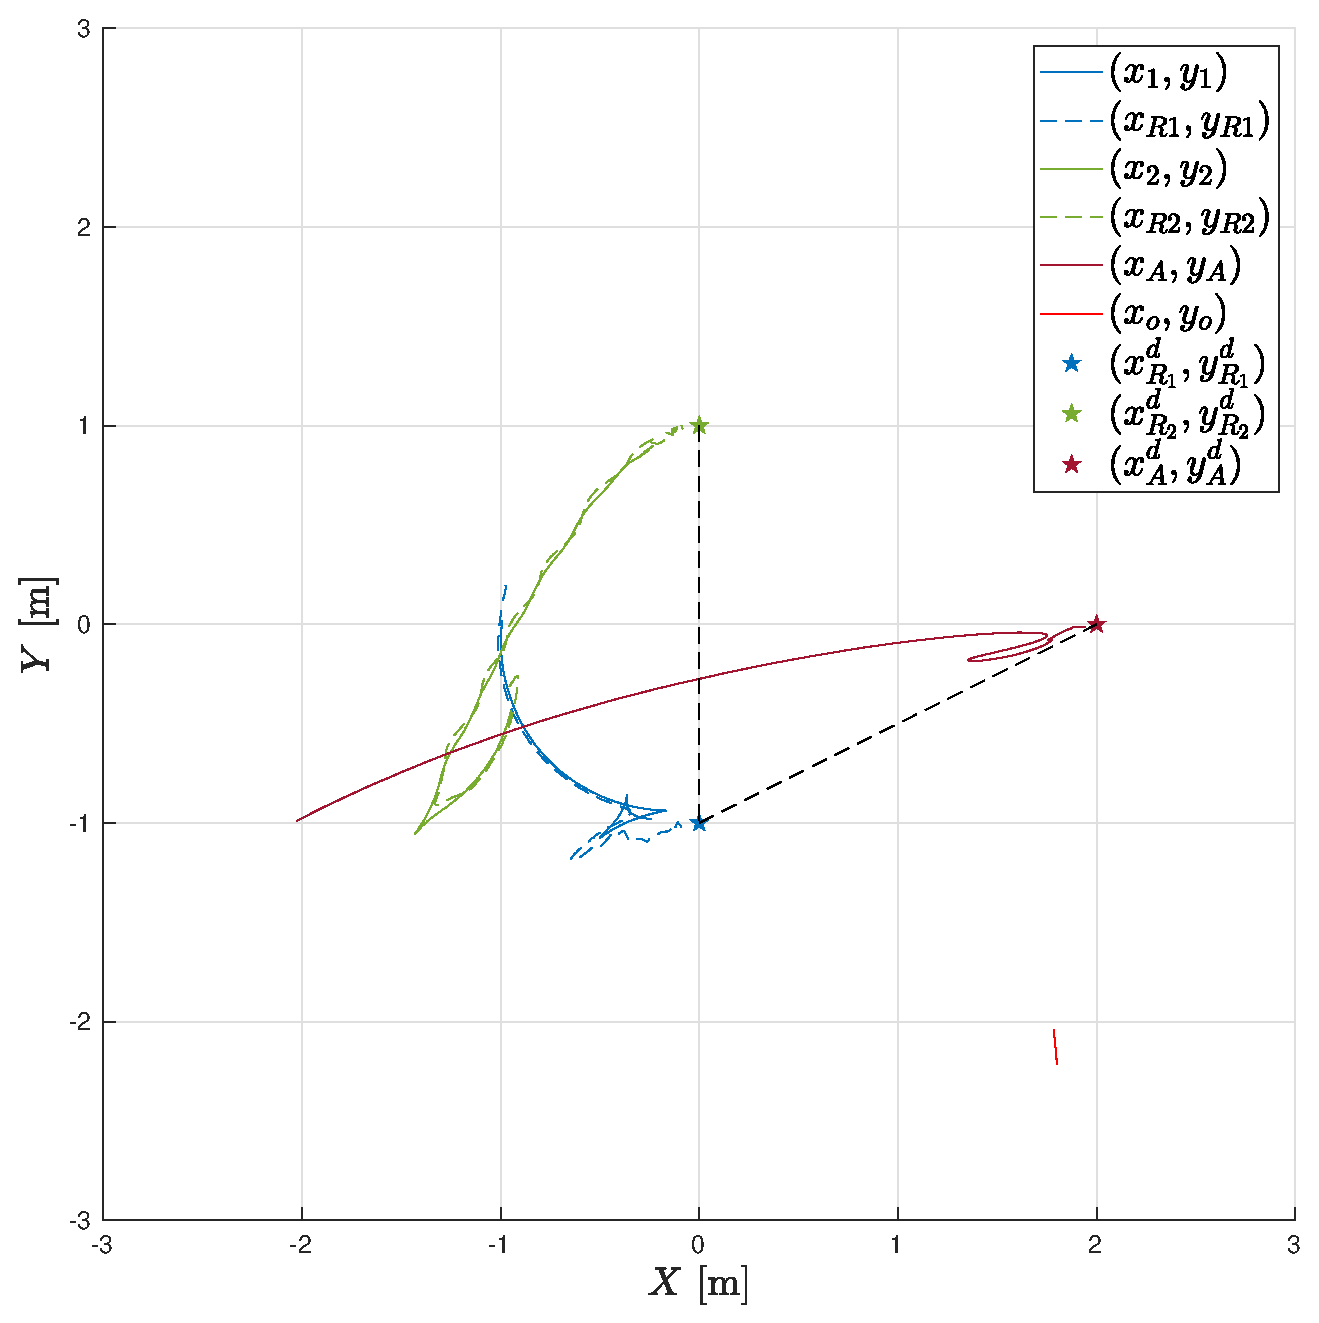
\includegraphics[width=\linewidth]{images/experiment/dynamic_obstacles/dynamicObst_exp_far.eps}
         \caption{$\SI{0}{\second} \leq  t \leq \SI{11}{\second}$}
    \end{subfigure}
    \begin{subfigure}[b]{0.32\columnwidth}
        \centering
        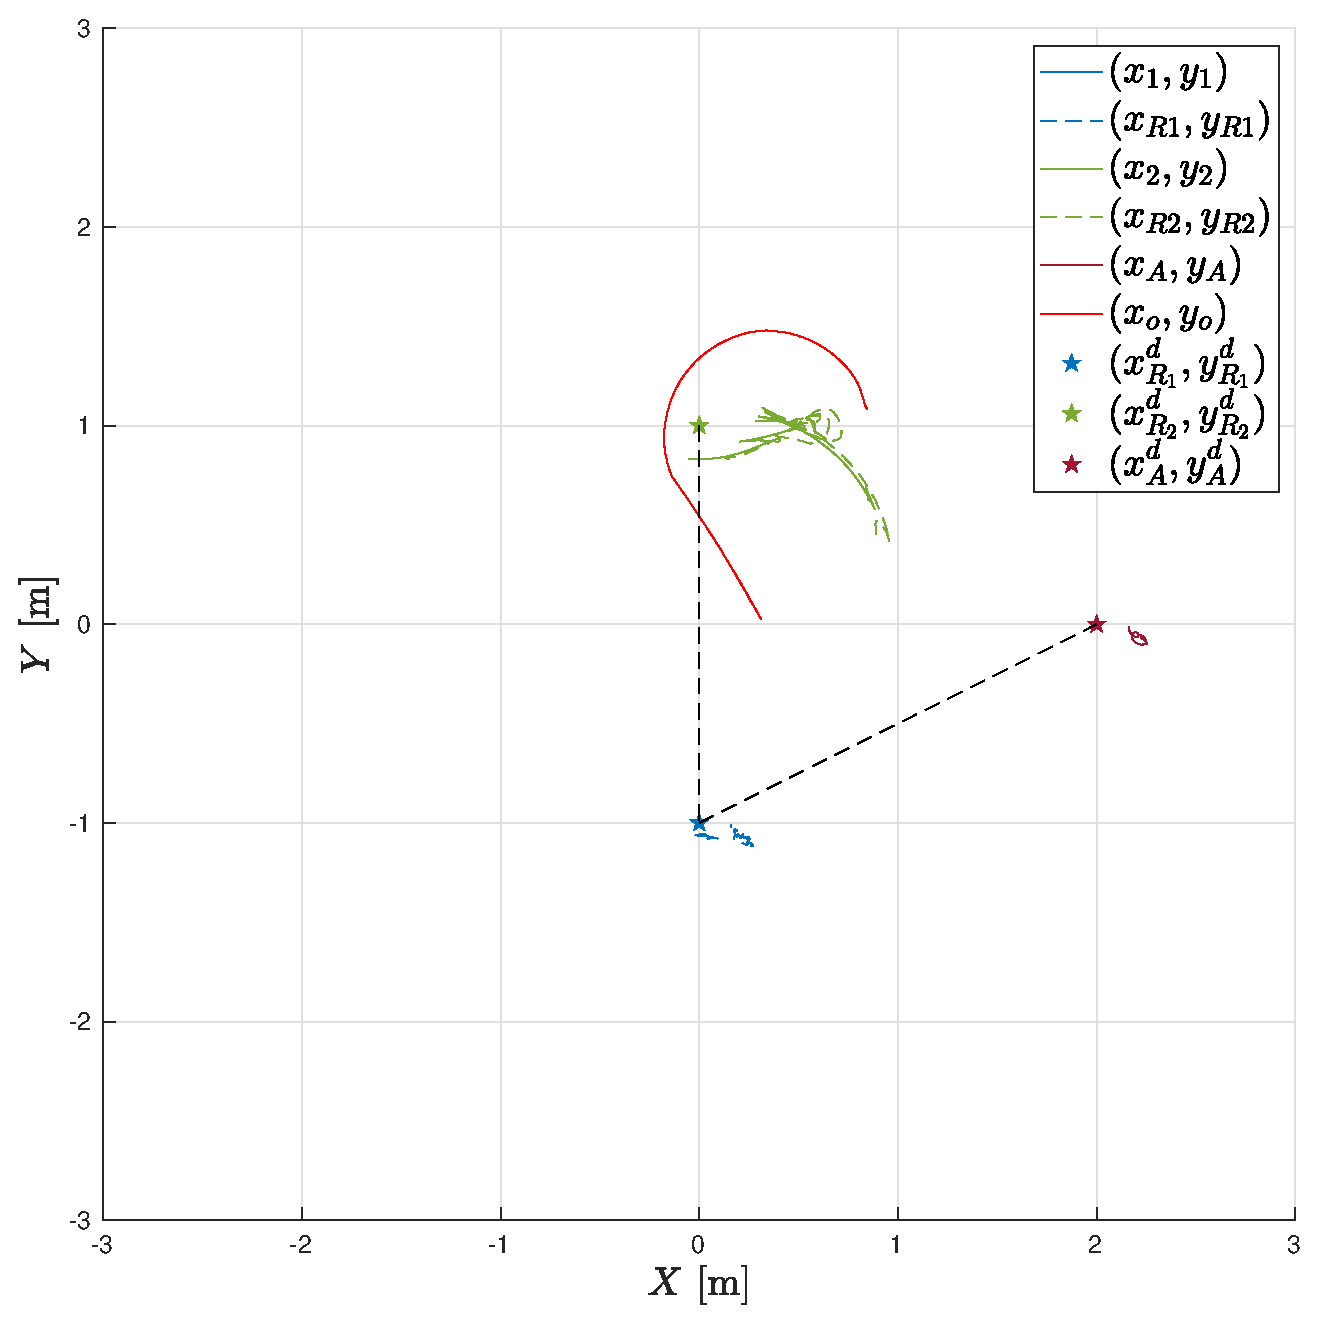
\includegraphics[width=\linewidth]{images/experiment/dynamic_obstacles/dynamicObst_exp_closeR2.eps}
         \caption{$\SI{31}{\second} \leq  t \leq \SI{42}{\second}$}
    \end{subfigure}
    \begin{subfigure}[b]{0.32\columnwidth}
        \centering
        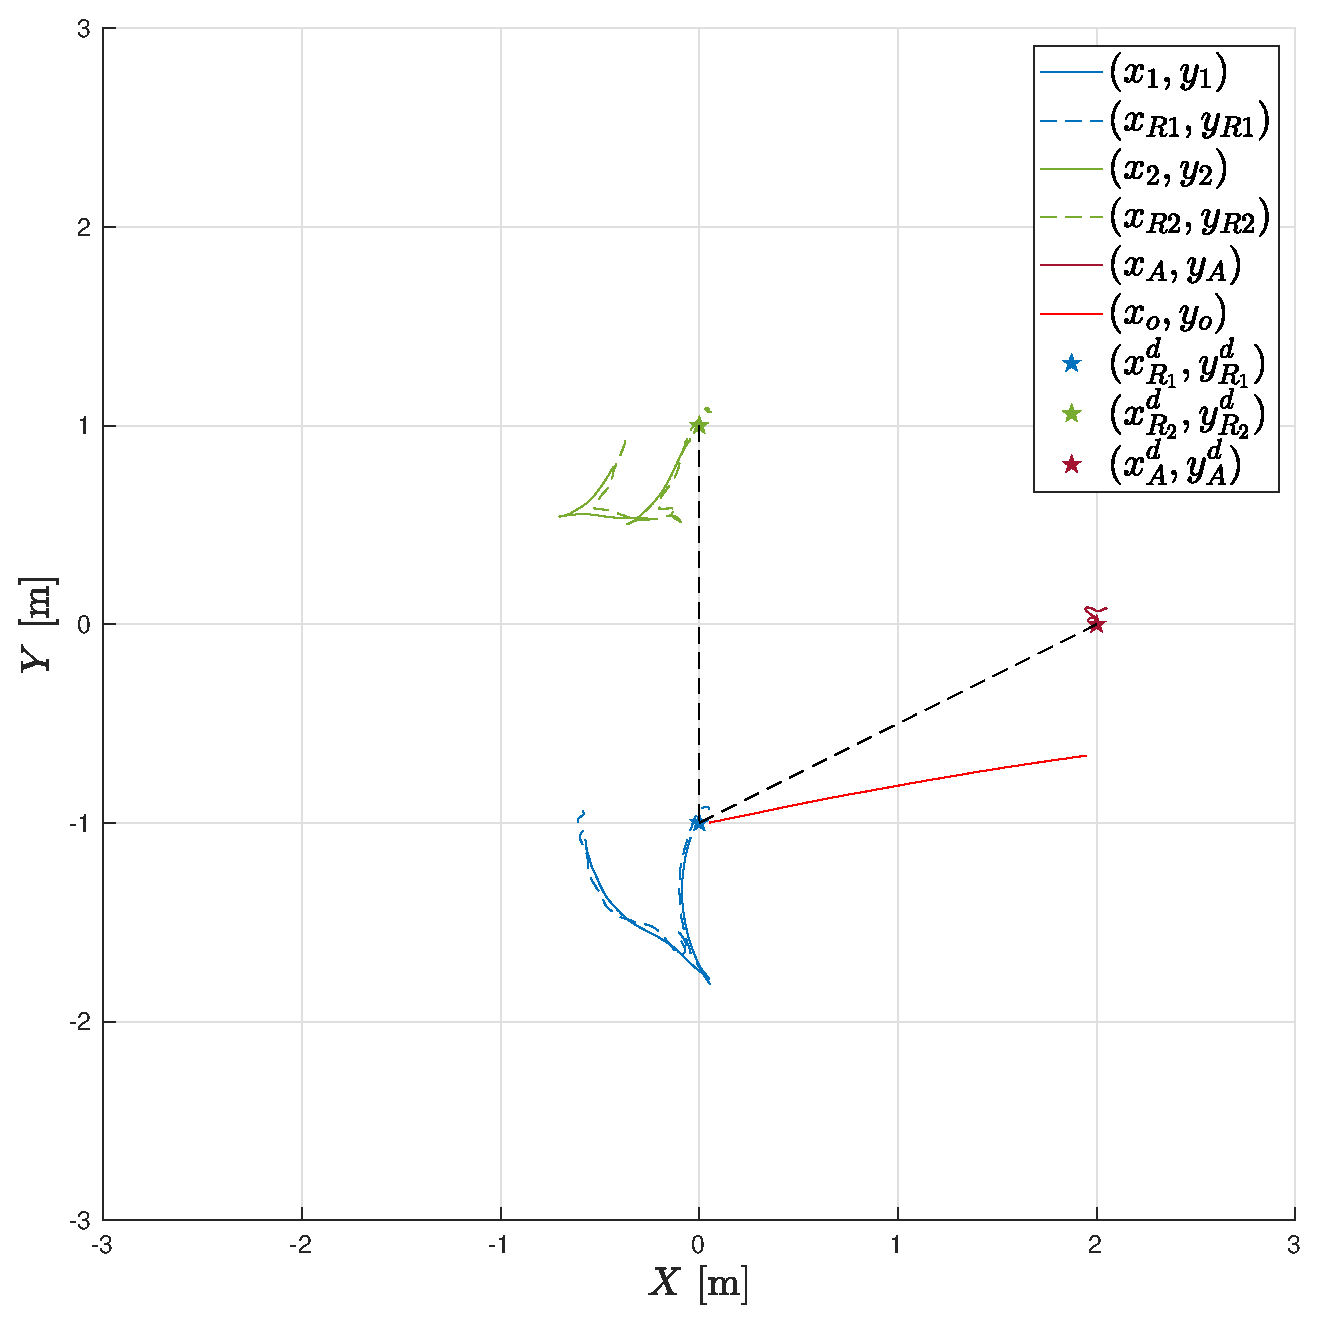
\includegraphics[width=\linewidth]{images/experiment/dynamic_obstacles/dynamicObst_exp_closeR1.eps}
        \caption{$\SI{56}{\second} \leq  t \leq \SI{63}{\second}$}
    \end{subfigure}
    \vspace{-0.2cm}
    \caption{\textcolor{red}{TODO}}
\end{figure}

\section{Conclusion}
\label{sec:conclusion}

\dots

\bibliography{bibliography}    % bib file to produce the bibliography
                           % with bibtex (preferred)

\end{document}
